\documentclass[12pt,a4paper,titlepage]{article}
\usepackage[T1]{fontenc}
\usepackage[utf8]{inputenc}
\usepackage{lmodern}
\usepackage[english]{babel}
\usepackage{geometry}
\geometry{margin=2.5cm}
\usepackage{graphicx}
\usepackage{amsmath}
\usepackage{amssymb}
\usepackage{booktabs}
\usepackage{tabularx}
\usepackage{enumitem}
\usepackage{natbib}
\usepackage{algorithm}
\usepackage{algpseudocode}
\usepackage{xcolor}
\definecolor{linknavy}{RGB}{0,51,102}
\usepackage[colorlinks=true,linkcolor=linknavy,citecolor=linknavy,urlcolor=linknavy]{hyperref}
\hypersetup{
  pdftitle={Reward Shape and Frame Stacking in DQN: A Reward x Observation Ablation in Multi-Objective Grid Survival},
  pdfauthor={Philipp Merz}
}
\usepackage{caption}
\captionsetup{font=small,labelfont=bf}
\usepackage{microtype}
\setlength{\emergencystretch}{3em}

\begin{document}

\begin{titlepage}
\centering
\vspace*{\stretch{0.8}}

{\large\scshape Eindhoven University of Technology\par}

\vspace{\stretch{1}}

\noindent\rule{\textwidth}{0.4pt}
\vspace{0.7\baselineskip}

{\LARGE\bfseries Reward Shape and Frame Stacking in DQN\par}

\vspace{0.6\baselineskip}

{\Large A Reward $\times$ Observation Ablation in\\[0.3\baselineskip]
Multi-Objective Grid Survival\par}

\vspace{0.7\baselineskip}

\noindent\rule{\textwidth}{0.4pt}

\vspace{1.2\baselineskip}

{\large\scshape Bachelor's Thesis\par}

\vspace{\stretch{1.4}}

{\Large Philipp Merz\par}

\vspace{1.5\baselineskip}

{\large Supervisor: Maxence Delorme\par}

{\normalsize Tilburg University\par}

\vspace{\stretch{1.6}}

{\large 2026\par}

\vspace*{\stretch{0.8}}
\end{titlepage}

\begin{abstract}
In this thesis we study two design choices that strongly affect how a deep reinforcement learning agent learns: the reward function it is asked to optimize, and how much short-term history of the world it observes at each step. The first determines what counts as good behavior. The second determines whether the agent can perceive motion at all, since a single snapshot only reveals position, but not direction or speed. To examine that interaction we built a small grid-world survival game in which an agent must eat to avoid starvation, evade enemies, and optionally take refuge in shelters, and trained a Deep Q-Network agent on this task while varying the reward function and the observation (either the current frame, or the four most recent frames concatenated). Our results show that frame stacking is not universally beneficial. It improved survival when maximizing the reward required actually surviving, but degraded it under two reward designs that admit easier ways to accumulate reward without surviving. Under those misspecified rewards, the agent used the additional perceptual capability to collect more reward at the cost of staying alive. The agent that combined the well-specified reward with the four-frame observation reached a survival level comparable to a scripted reference policy hand-written for the task. These findings are specific to our environment, but suggest that observation-side and reward-side design decisions cannot be treated as independent.
\end{abstract}

\tableofcontents
\newpage

% =============================================================================
\section{Introduction}
\label{sec:introduction}
% =============================================================================

In reinforcement learning, an agent learns a policy (a mapping from observations of an environment to actions) by interacting with that environment. At each step it observes the current state, takes the action prescribed by its current policy, and receives a reward signaling how good the choice was. The agent's objective is to discover a policy that, over time, accumulates as much reward as possible. The reward function therefore defines what the agent considers good behavior. When the task is simple, a single reward signal at the end of each episode can suffice. When the task is complex and combines several competing objectives (making progress, avoiding harm, managing limited resources), a single end-of-episode signal is too coarse, since the agent has no way to tell which of the many low-level actions taken during the episode contributed to the outcome.

The standard response is reward shaping, where the agent receives a small reward at every step in addition to or instead of the terminal signal, computed as a weighted sum of several quantities that proxy for the designer's intent. Make progress toward the goal, gain reward. Take damage, lose reward. Stay near a safe area, gain reward. Each weighted component pulls the agent's behavior in some direction, and collectively they are meant to steer it toward the intended overall policy. In practice, finding weights that produce the intended behavior is one of the hardest parts of training agents for multi-objective embodied control tasks such as legged-robot locomotion and aerial navigation \citep{Hwangbo2019, Hwangbo2017}.

Small changes in relative weights can lead the agent to qualitatively different behaviors, including policies that maximize the shaped reward without producing what the designer had in mind. A reward designed to encourage the agent to forage may instead teach it to hover near food without eating it, because hovering pays continuously while eating ends the reward stream. This kind of mismatch between the shaped reward and the behavior it was meant to encode is known as reward hacking \citep{Amodei2016}. From the agent's perspective, no error has been made. It is simply optimizing the function it was given.

A second design choice, parallel to the reward, concerns what the agent perceives at each step. An environment that exposes only the current state allows the agent to access positional information, but not motion. Whether an approaching object is moving toward or away from the agent, for instance, cannot be inferred from a single snapshot. The standard remedy is to give the agent a short history of recent observations rather than only the most recent one, an approach known as frame stacking \citep{Mnih2013}. With recent history available, the agent can in principle learn to infer derived quantities, such as velocity, directly from its input.

These two design axes, reward and observation, are routinely tuned together when training agents but are rarely studied as interacting variables in their own right. We approached the experiments described below with the expectation that providing more observation history via frame stacking should at worst do nothing, since extra information that the agent does not need can simply be ignored. We therefore hypothesized that the combination of the cleanest available reward design and the richer observation would produce the strongest agent, and that adding observation history would at worst be neutral under the other reward designs. The experiments will show that this expectation held only in part, and that the effect of frame stacking on survival depends on the shape of the reward in a surprising way.

To investigate this question we constructed a small grid-world survival environment in which an agent must manage hunger, evade enemies, and optionally take refuge in shelters. The environment is deliberately simple, exposing only the mechanisms relevant to the reward-shaping question (competing objectives, a per-step managing of hunger and progress, and event-driven rewards for eating and being hit) and removing everything not relevant (rich action spaces, procedurally generated worlds, multi-agent interactions). On this environment we train one fixed agent architecture under several reward configurations and two observation depths, and compare its behavior against that of a hand-written reference policy that captures the intended use of the environment. The source code and experiment configurations are available at \url{https://github.com/philippmerz/rl-thesis}. The investigation is constrained to a single environment and a modest training budget, and the conclusions we draw are correspondingly modest. The detailed experimental design and methodology are given in Section~\ref{sec:experiments}.

The remainder of the thesis is organized as follows. Section~\ref{sec:related_work} surveys the related literature. Section~\ref{sec:background} reviews the technical background on reinforcement learning, deep Q-learning, and reward shaping. Section~\ref{sec:environment} describes the survival environment in detail and explains why we built a custom environment rather than reuse an existing benchmark. Section~\ref{sec:architecture} details the agent we trained. Section~\ref{sec:experiments} presents the experimental design, failure-mode analysis, reward configurations, and the main ablation. Section~\ref{sec:discussion} reports the results and discusses them. Section~\ref{sec:conclusion} concludes.

% =============================================================================
\section{Related Work}
\label{sec:related_work}
% =============================================================================

In contemporary deep reinforcement learning (RL) practice, reward shaping refers broadly to constructing a per-step reward as a weighted sum of components that each proxy for some aspect of the designer's intent. Published reward functions for multi-objective embodied control commonly assemble several such components. The reward functions of \citet{Hwangbo2019} for legged-robot locomotion and \citet{Hwangbo2017} for quadrotor flight weigh forward progress, attitude stability, energy expenditure, smoothness, and other quantities against each other. \citet{Loquercio2021} use a comparable hand-tuned, multi-term objective for agile drone navigation. Across these examples the weights are hand-tuned, and their calibration is widely reported as one of the practical bottlenecks in training such policies. This thesis studies what happens when this reward-tuning task is paired with a second design decision on the observation side.

\citet{Amodei2016} catalogued reward hacking as one of several concrete safety failure modes that emerge when learned policies optimize a proxy reward instead of the underlying objective directly. The phenomenon predates deep RL by decades. \citet{Lehman2020} collect a wide range of earlier examples from evolutionary computation and artificial life, including virtual creatures evolved to jump that instead learned to exploit bugs in the physics simulation to gain height without ever actually jumping. Whether such exploits are found at all depends on the agent's capability. \citet{Pan2022} make this dependence empirically concrete. Holding the reward misspecification fixed while varying model size, action-space resolution, observation noise, and training time, they find that more capable agents do better on the misspecified reward they were trained against but worse on the objective the reward was meant to capture, sometimes crossing thresholds at which the behavior changes abruptly. We later use this reward-capability interaction framework to interpret our own experimental findings.

Beyond the reward and the agent's capability, the environment in which the agent is trained and tested is a third design lever. It must expose the phenomena under investigation in a form that can be measured cleanly. So-called gridworlds, simulated 2D-grid environments, have long served this purpose, since they isolate phenomena that are hard to study in more realistic and complex settings. \citet{Leike2017} introduce a suite of safety-focused gridworlds that expose common ways RL agents misbehave. Their environments include settings where the agent finds unintended shortcuts to high reward, settings where it causes collateral damage in pursuit of its objective, and settings where it performs badly when the deployment environment differs from the one it trained in. Several are explicit reward-hacking benchmarks of the kind described above. \citet{Hafner2022} provide the Crafter benchmark, a multi-objective survival gridworld with a procedurally generated layout each episode in which the agent forages for food and water, sleeps, fights enemies, and builds shelter. The MiniGrid framework of \citet{ChevalierBoisvert2023} is goal-oriented rather than survival-based, tasking the agent with reaching a target tile or retrieving an object across a modular set of layouts. The NetHack Learning Environment \citep{Kuttler2020} extends the survival paradigm to a much larger action space and far longer episodes. The environment used in this thesis is a leaner instance of this survival design.

Alongside the choice of environment is the choice of what the agent perceives within it. Frame stacking, the observation-side variable of our experiments, was introduced in the original deep Q-learning work \citep{Mnih2013} to give a standard feed-forward network access to short-term motion information that a single frame cannot convey. The canonical alternative is to use recurrent network architecture instead. \citet{Hausknecht2015} introduce DRQN, which extends DQN with such a recurrent component and remains the standard reference for the recurrent approach.

All of these design choices ultimately have to be exercised at some compute scale. The single-laptop training budget used in this thesis is supported by recent work showing that algorithmic choices can substitute for large-scale compute in deep Q-learning. \citet{ObandoCeron2021} revisit the deep Q-learning baseline of \citet{Hessel2018} under more careful evaluation. \citet{Schwarzer2023}, \citet{ObandoCeron2023}, and \citet{Clark2024} demonstrate that consumer-grade hardware can match results previously requiring large-scale compute, through algorithmic refinements such as smaller networks and more efficient use of replay. These results inform the choice of agent and training budget in Section~\ref{sec:architecture}.

% =============================================================================
\section{Background}
\label{sec:background}
% =============================================================================

\subsection{Reinforcement Learning Fundamentals}

We formulate the task as a Markov Decision Process (MDP) defined by a tuple $(S, A, P, R, \gamma)$: state space $S$, action space $A$, transition function $P(s' \mid s, a)$, reward function $R(s, a, s')$, and discount factor $\gamma \in [0, 1)$ \citep{SuttonBarto2018}.

The agent interacts with the environment in discrete time steps $t = 0, 1, 2, \ldots$, receiving reward $r_t \in \mathbb{R}$ at each step. The goal is to find a policy $\pi: S \to A$ that maximizes the expected discounted return $G_t = \sum_{k=0}^{\infty} \gamma^k r_{t+k+1}$. The action-value function
\begin{equation}
Q^\pi(s, a) = \mathbb{E}_\pi\!\left[G_t \mid s_t = s,\; a_t = a\right]
\end{equation}
gives the expected return of taking action $a$ in state $s$ and following $\pi$ thereafter. The optimal action-value function $Q^*(s, a) = \max_\pi Q^\pi(s, a)$ satisfies the Bellman optimality equation:
\begin{equation}
Q^*(s, a) = \mathbb{E}\!\left[r_t + \gamma \max_{a'\in A} Q^*(s_{t+1}, a')\right],
\end{equation}
where $s_{t+1}$ is the successor state reached after taking $a$ in $s$.

Q-learning estimates $Q^*$ directly through temporal difference (TD) updates:
\begin{equation}
Q(s_t, a_t) \leftarrow Q(s_t, a_t) + \alpha\!\left[r_t + \gamma \max_{a'} Q(s_{t+1}, a') - Q(s_t, a_t)\right],
\end{equation}
where $\alpha$ is the learning rate. The bracketed quantity is the TD error $\delta_t$. These updates assume we can store and update a $Q$-value for every state-action pair, which is feasible only when the state space is small enough to enumerate.

\subsection{Deep Q-Networks}

Deep Q-Networks (DQN) \citep{Mnih2013, Mnih2015} address this limitation by approximating $Q^*$ with a neural network $Q(s, a; \theta)$ parameterized by weights $\theta$.

Two mechanisms stabilize training. First, instead of sampling temporally correlated consecutive state transitions, which would violate the optimizer's i.i.d. data prerequisite, \emph{experience replay} stores transitions $(s, a, r, s')$ in a buffer and samples mini-batches uniformly. Second, a \emph{target network} with parameters $\theta^-$ provides stable TD targets. The loss for a sampled transition is:
\begin{equation}
L(\theta) = \left[r + \gamma \max_{a'} Q(s', a'; \theta^-) - Q(s, a; \theta)\right]^2.
\end{equation}
The target parameters $\theta^-$ are periodically copied from $\theta$.

Exploration uses an $\varepsilon$-greedy policy: with probability $\varepsilon$ a random action is taken, otherwise the greedy action $\arg\max_a Q(s, a; \theta)$.

Vanilla DQN as described above has known weaknesses, and a number of extensions have been proposed to address them individually. The next subsection describes the four such extensions that our agent incorporates.

\subsection{DQN Extensions}
\label{sec:dqn_extensions}

The first weakness is that DQN systematically overestimates action values. The target uses $\max_{a'} Q(s', a'; \theta^-)$, so any positive estimation noise in $Q$ is preferentially picked up by the $\max$ operator and biases the target upward. Double DQN \citep{vanHasselt2016} decouples action selection from action evaluation:
\begin{equation}
y = r + \gamma\, Q\!\left(s',\; \arg\max_{a'} Q(s', a'; \theta);\; \theta^-\right).
\end{equation}
The online network selects the maximizing action, and the target network evaluates it.

A second concern is that the network has to learn an explicit $Q$-value for every state-action pair, even in states where the action choice barely affects the outcome. The Dueling architecture \citep{Wang2016} factors the $Q$-function into a state value $V(s)$ and an action advantage $A(s, a)$:
\begin{equation}
Q(s, a) = V(s) + A(s, a) - \frac{1}{|A|}\sum_{a'} A(s, a'),
\end{equation}
where $|A|$ is the number of actions. The decomposition lets the network learn $V(s)$ without separately evaluating each action, which helps in states where the action choice has little effect on the value.

The third extension concerns how transitions are sampled from the replay buffer. Uniform sampling treats every transition the same, but transitions with large TD error carry more learning signal per sample. Prioritized experience replay (PER) \citep{Schaul2016} samples transitions in proportion to their TD-error magnitude, revisiting surprising transitions more often. The sampling probability of transition $i$ is
\begin{equation}
P(i) = \frac{p_i^\alpha}{\sum_k p_k^\alpha}, \quad p_i = |\delta_i| + \epsilon_p,
\end{equation}
where $\alpha$ controls prioritization strength and $\epsilon_p$ is a small constant ensuring nonzero probability. Non-uniform sampling introduces bias, which is corrected by importance-sampling (IS) weights
\begin{equation}
w_i = \left(\frac{1}{N \cdot P(i)}\right)^\beta\!\bigg/\; \max_j w_j,
\end{equation}
where $N$ is the number of stored transitions and $\beta$ is annealed from a starting value to 1 during training, gradually applying the full bias correction.

A fourth extension addresses the slow propagation of reward through single-step bootstrapping. $n$-step returns \citep{Sutton1988, SuttonBarto2018} accumulate rewards over $n$ consecutive steps before bootstrapping:
\begin{equation}
\label{eq:nstep}
R_t^{(n)} = \sum_{k=0}^{n-1} \gamma^k r_{t+k+1} + \gamma^n \max_{a'} Q(s_{t+n}, a'; \theta^-).
\end{equation}
This propagates reward information faster at the cost of increased variance. Moderate values of $n$ (typically 2--5) improve learning speed in practice.

\citet{Hessel2018} combined six such extensions into a single agent under the name Rainbow. The six are Double DQN, Dueling, PER, multi-step returns, distributional RL (C51), and NoisyNet. Their ablation showed each component contributes, with PER and multi-step returns providing the largest individual gains. We adopt the four techniques outlined above, but omit distributional RL and NoisyNet because of implementation complexity.

\subsection{Training Stability Techniques}
\label{sec:stability}

Beyond the algorithmic extensions above, two further design choices stabilize the optimization itself.

The original DQN copies $\theta$ to $\theta^-$ every $C$ steps, which creates discontinuities in the target. The soft (Polyak) target update \citep{Lillicrap2016} replaces the hard copy with an exponential moving average, updating the target at every step:
\begin{equation}
\theta^- \leftarrow (1 - \tau)\,\theta^- + \tau\,\theta,
\end{equation}
with a small $\tau$. This produces smoother target evolution rather than the periodic discontinuities of the hard copy.

Batch normalization, the standard choice in supervised deep learning, is unreliable in deep RL because the data distribution is non-stationary and effective batch sizes are small. LayerNorm \citep{Ba2016} instead normalizes across features within each sample, independently of the batch. \citet{Gallici2024} show empirically across Atari-game ablations that LayerNorm improves deep $Q$-learning performance over batch normalization in this regime.

\subsection{Reward Shaping}
\label{sec:reward_shaping_bg}

Reward shaping refers to the practice of designing a per-step reward signal that decomposes the intended overall objective into a sum of smaller, denser terms. When the task has competing sub-objectives, or when the terminal reward is too sparse for the agent to learn from in reasonable time, a hand-tuned dense reward gives step-by-step feedback that proxies the designer's intent. The weights on the individual components are design parameters whose calibration determines whether the learned policy matches that intent.

Formally, a shaped reward is just another scalar function of state, action, and successor state. The agent's only objective is to maximize its expected discounted sum. Whether that sum coincides with the designer's intent depends entirely on whether the chosen function does. Most ad-hoc shaping is a weighted combination of heuristic components, each separately encoding a fragment of good behavior. The agent does not see those fragments as parts of an aggregate goal. It sees only a scalar at each step and optimizes the total. Any combination of weights that admits a higher-scoring strategy than the intended one creates a target for the agent to find, but whether the agent actually finds it depends on its capability.

\citet{Pan2022} make this dependence concrete. Holding misspecified rewards fixed while varying agent capability (model capacity, action-space resolution, observation noise, and training time), they find that more capable agents systematically earn higher \emph{proxy} reward and lower \emph{true} reward, in some cases crossing capability thresholds at which behavior changes abruptly. Reward hacking, in this view, is not a property of the reward function alone but a property of the function together with the agent's capability to reach its loopholes. This makes for an unintuitive phenomenon: the same reward can produce intended behavior under a weak agent and pathological behavior under a stronger one.

Throughout the rest of this thesis, we use the term \emph{leaky} informally to describe a reward function whose episode return can be inflated by behavior that does not serve the intended objective. An imperfect reward \emph{leaks} return to behaviors outside what it was meant to incentivize, the way a leaky pipe loses water to places it was not meant to flow. The cleaner the reward (in the sense of admitting fewer such loopholes), the smaller the gap between proxy reward and true objective should be, and the less reward hacking should be possible.

% =============================================================================
\section{Environment}
\label{sec:environment}
% =============================================================================

The survival environment used throughout this thesis was built specifically for the work, implemented from scratch rather than as a fork or extension of an existing library. We chose this route because the closest available alternatives did not match the research question cleanly. The Crafter benchmark \citep{Hafner2022} expands the survival theme into a much larger 17-action task with crafting, inventory, and 22 achievements, most of which are tangential to the reward-shape question studied here. MiniGrid \citep{ChevalierBoisvert2023} is narrower, but its built-in environments are explicitly goal-oriented, framed around reaching a target tile or picking up an object rather than indefinite survival under competing pressures. A custom implementation also lets the environment step fast enough that each of the twenty-four training runs in our ablation completes within a few hours on a consumer GPU. Figure~\ref{fig:env_screenshot} shows a representative mid-episode snapshot. The subsections below describe the design in detail.

\begin{figure}[h]
\centering
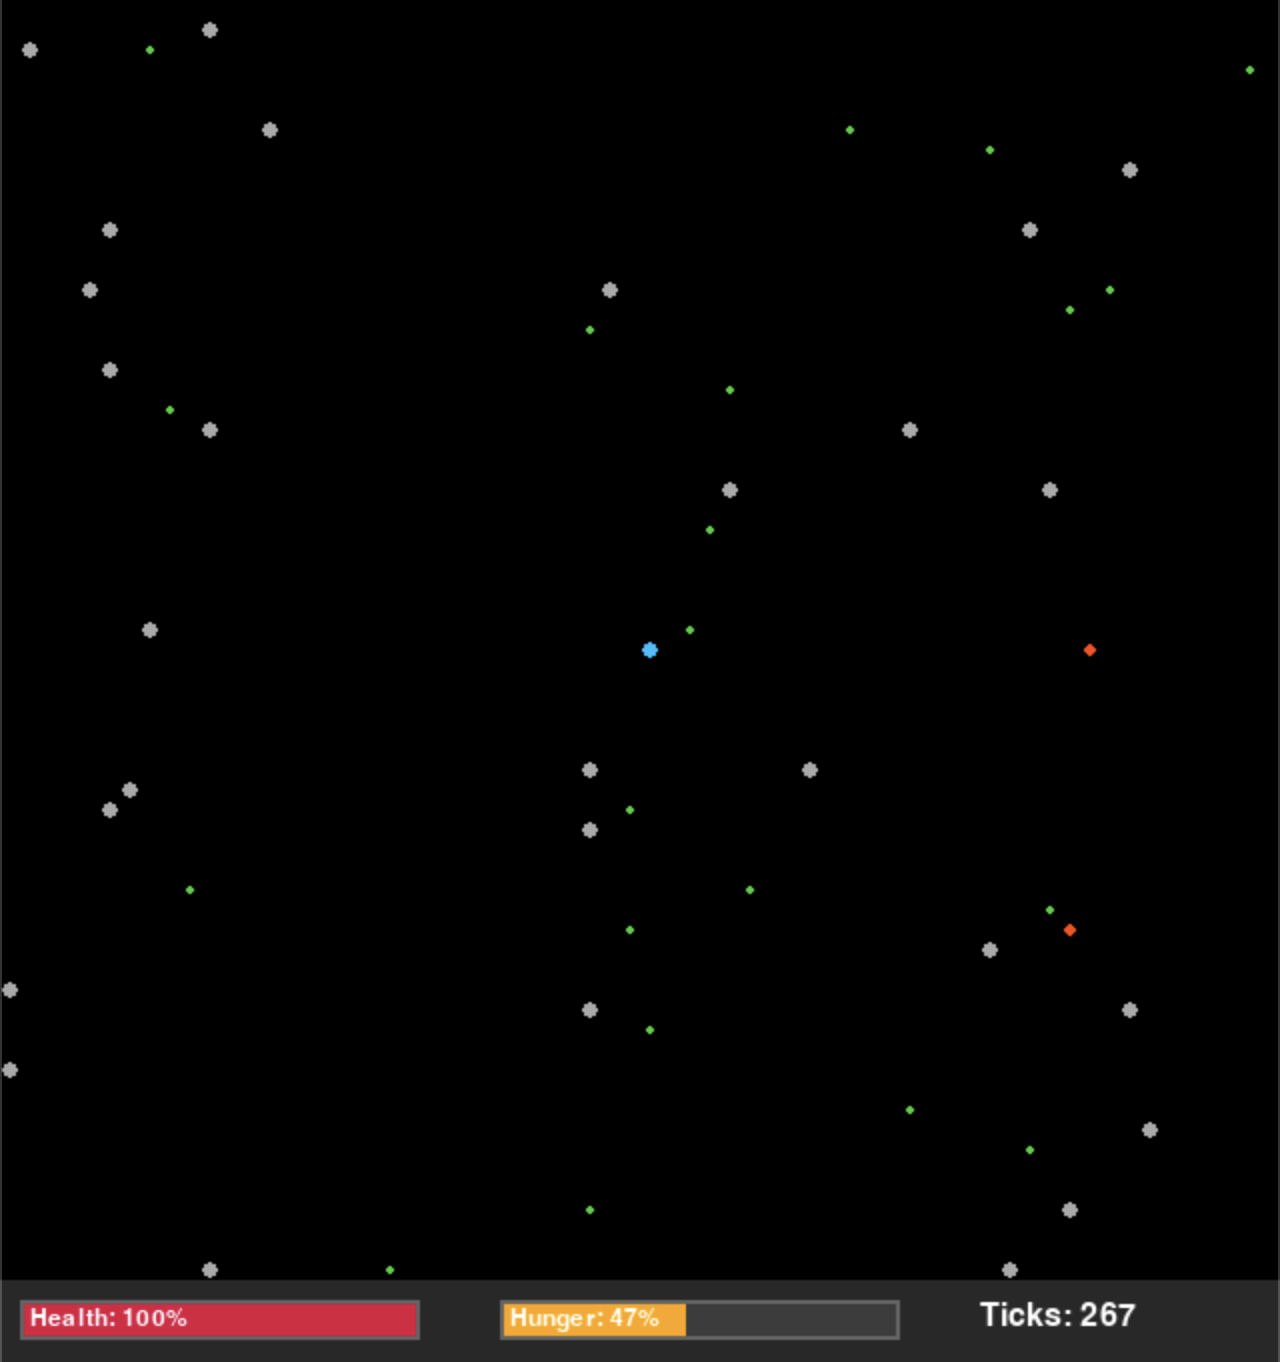
\includegraphics[width=0.65\textwidth]{figures/environment.png}
\caption{Screenshot of the survival environment. The agent (blue dot) is near the grid center. Two enemies (red dots) are visible to the east. Food items (small green dots) are scattered across the grid and replenish stochastically over time. Shelters (large gray dots) are placed once at episode start and remain fixed. The bottom bar reports current health and hunger, and current tick count.}
\label{fig:env_screenshot}
\end{figure}

\subsection{World Design}
\label{sec:world_design}

The environment is a $64 \times 64$ bounded grid with discrete time steps. An episode ends when the agent dies (health reaches zero) or when an episode cap on the number of ticks is reached. The world contains four entity types.

\paragraph{Agent.} A single agent with two resource bars: health $h$ and hunger $u$, both with maximum value $h_\text{max} = u_\text{max} = 100$. The agent spawns at the grid center with both bars full. Hunger depletes by $0.2$ per tick and by an additional $0.5$ when moving. When hunger reaches zero, the agent starves and loses $0.5$ health per tick. When hunger exceeds the threshold $u_\text{thresh} = 0.3$ ($30\%$ of maximum), health regenerates at $0.5$ per tick up to the cap.

\paragraph{Enemies.} Mobile entities that deal 15 damage on contact (Manhattan distance $\leq 1$). Each tick, an enemy moves with probability 0.5. Within a vision range of 3 (Manhattan distance), enemies pursue the agent along the axis of greatest distance. Outside this range, they move randomly. Enemies cannot enter shelter tiles or tiles occupied by another enemy. The world supports up to 8 enemies simultaneously, with roughly a third of this capacity present at episode start. New enemies appear with probability 0.01 per tick.

\paragraph{Food.} Stationary items that restore 20 hunger when consumed by stepping onto their tile. Up to 36 food items exist simultaneously, with half present at episode start. New food appears with probability 0.05 per tick.

\paragraph{Shelters.} 
Stationary tiles generated at episode start with density 0.01 per cell (approximately 41 shelters per episode). While in a shelter, the agent takes no damage from enemies. Shelters do not protect against starvation.

Each episode uses a different random seed, producing a unique shelter layout and initial entity placement. Enemy and food spawning continues throughout the episode, maintaining population pressure.

\subsection{Observation Space}

The agent observes through a $15 \times 15$ window (radius $r_\text{obs} = 7$) centered on the agent. The observation consists of three binary spatial channels:
\begin{enumerate}[nosep]
\item Enemy presence
\item Food presence
\item Shelter presence
\end{enumerate}
Cells outside the grid boundary are zero. Three scalar features are appended: $\frac{h}{h_\text{max}}$, $\frac{u}{u_\text{max}}$, and a binary shelter indicator. The full single-frame observation is a $678$-dimensional vector ($3 \times 15 \times 15 = 675$ spatial entries plus $3$ scalar features). The 4-frame stacked variant introduced as the observation-side ablation in Section~\ref{sec:ablation} concatenates the spatial channels of the four most recent frames, raising the spatial channel count from $3$ to $12$. The spatial component therefore grows by an exact factor of $4$ (from $675$ to $2{,}700$), but the three scalar features are taken from the current frame only, since they reflect the cumulative state of the agent and do not benefit from temporal stacking. Thus, the total observation dimension grows from $678$ to $2{,}703$, by a factor of $2703 / 678 \approx 3.99$. Figure~\ref{fig:obs_space} illustrates the layout.

\begin{figure}[h]
\centering
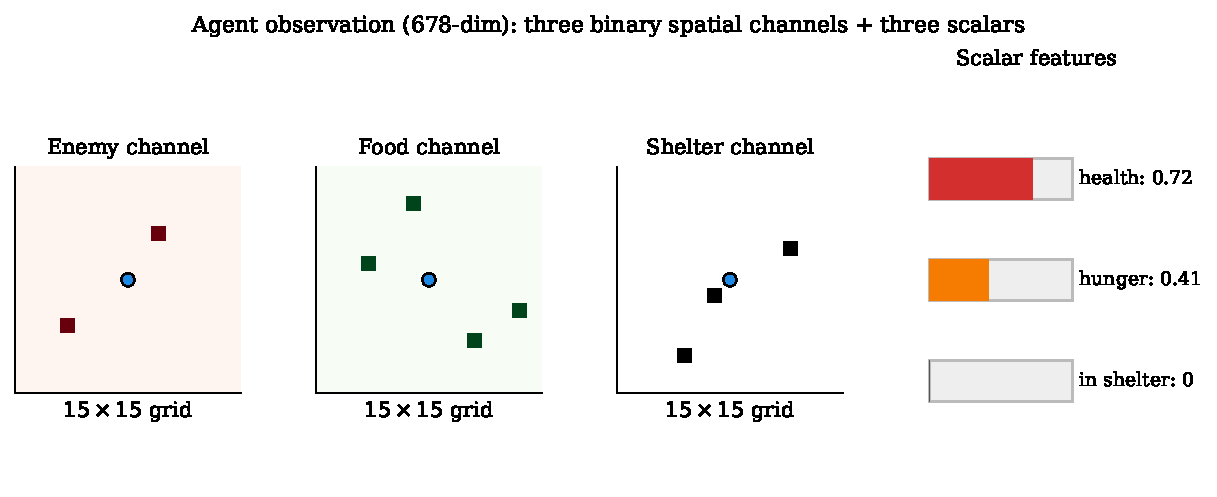
\includegraphics[width=\linewidth]{figures/observation_space}
\caption{Observation structure. The agent (blue dot at the window center) sees three binary $15 \times 15$ grids corresponding to enemy, food, and shelter presence within radius 7, plus three scalar features summarizing the agent's internal state. Section~\ref{sec:ablation} crosses this single-frame observation with a 4-frame stacked variant ($12$ spatial channels) as the observation-side ablation.}
\label{fig:obs_space}
\end{figure}

\subsection{Action Space}

The agent has five discrete actions: stay in place, or move one cell up, down, left, or right. Movement is clamped to the grid boundaries.

\subsection{Reward Structure}
\label{sec:reward_structure}

The reward at each step is a weighted sum of up to eleven components:
\begin{equation}
\label{eq:reward}
\begin{aligned}
r_t ={}& w_\text{food}\, i_t^{(\text{eat})}
    + w_\text{edm}\, d_t^{(\text{e})}
    + w_\text{sdm}\, d_t^{(\text{s})}
    + w_\text{death}\, i_t^{(\text{die})} \\
& + w_\text{hunger}\, i_t^{(\text{low})}
    + w_\text{hprop}(1 - u_t)
    + w_\text{tick} \\
& + w_\text{fprox}\, \Delta\phi_t^{(\text{f})}
    + w_\text{eprox}\, \Delta\phi_t^{(\text{e})}
    + w_\text{sprox}\, \Delta\phi_t^{(\text{s})} \\
& + w_\text{shelter}\, i_t^{(\text{safe})},
\end{aligned}
\end{equation}
where $w_{\cdot} \in \mathbb{R}$ are tunable scalar weights; $i_t^{(\text{eat})}, i_t^{(\text{die})}, i_t^{(\text{low})}, i_t^{(\text{safe})} \in \{0,1\}$ are binary indicators for food eaten, death, low hunger, and shelter safety; $d_t^{(\text{e})}$ and $d_t^{(\text{s})}$ are enemy damage and starvation damage; and $u_t \in [0, 1]$ is the hunger ratio.

Table~\ref{tab:default_rewards} lists all reward components and their baseline weights.

\begin{table}[h]
\centering
\caption{Reward components and baseline weights. Components marked ``disabled'' are set to zero in the baseline and activated in specific experimental configurations.}
\label{tab:default_rewards}
\small
\begin{tabular}{llr}
\toprule
Component & Condition & Baseline \\
\midrule
Food eaten ($w_\text{food}$)          & Agent steps on food tile              & $+5.0$ \\
Enemy damage ($w_\text{edm}$)         & Per unit of damage received           & $-0.1$ \\
Starvation damage ($w_\text{sdm}$)    & Per unit of starvation damage         & $-1.0$ \\
Death ($w_\text{death}$)              & Health reaches zero                   & $-10.0$ \\
Low hunger ($w_\text{hunger}$)        & Per tick when $u_t < u_\text{thresh}$ & disabled \\
Hunger proportional ($w_\text{hprop}$) & Continuous, scales with $(1 - u_t)$  & $-0.3$ \\
Food proximity ($w_\text{fprox}$)     & Change in closeness to nearest food this step    & $+0.1$ \\
Enemy proximity ($w_\text{eprox}$)    & Change in closeness to nearest enemy this step   & disabled \\
Shelter proximity ($w_\text{sprox}$)  & Change in closeness to nearest shelter this step & disabled \\
Shelter safety ($w_\text{shelter}$)   & Agent in shelter, enemy within distance 3 & $+0.1$ \\
Survival tick ($w_\text{tick}$)       & Per step alive                        & disabled \\
\bottomrule
\end{tabular}
\end{table}


The three proximity terms reward per-step changes in closeness to a target, rather than absolute closeness. For target type $x \in \{\text{f}, \text{e}, \text{s}\}$ (food, enemy, shelter), define the closeness score
\begin{equation}
\phi_t^{(x)} = \frac{dist_\text{max} - dist_t^{(x)} + 1}{dist_\text{max} + 1} \in [0, 1],
\end{equation}
where $dist_t^{(x)}$ is the Manhattan distance to the nearest visible entity of type $x$ and $dist_\text{max} = 2r_\text{obs}$ (maximum Manhattan distance to any cell within the observation radius). If no entity is visible, $\phi_t^{(x)} = 0$. The per-step closeness change $\Delta\phi_t^{(x)} = \phi_t^{(x)} - \phi_{t-1}^{(x)}$ is positive when the agent moved closer to the target in that step and negative when it moved away. We reward this per-step change rather than the absolute closeness because rewarding absolute closeness would also reward standing still next to a target (for example, hovering next to a food tile without eating it). The per-step change form gives zero reward for staying in place, so it only pays the agent for moving toward the target.

Two proximity terms can be conditionally turned on (gated) based on the hunger ratio, using a dedicated gating threshold $u_\text{gate}$. When conditional gating is enabled, the food proximity fires only when $u_t < u_\text{gate}$ (hungry) and the shelter proximity fires only when $u_t \geq u_\text{gate}$ (well-fed). This encodes a behavioral mode switch through the reward function: the agent receives a spatial indicator toward food when it needs to eat and toward shelter when it does not.

These components create competing pressures. Collecting food requires movement, which costs hunger and exposes the agent to enemies. Shelters neutralize enemy damage but provide no food. The hunger-proportional penalty grows every tick, creating urgency to eat that the agent cannot escape through passivity.

Another design consideration is the relative magnitude of continuous per-tick rewards versus sparse event rewards. A small per-tick reward that fires at every step can in aggregate exceed an infrequent event reward, biasing the agent toward passive survival rather than active foraging. Similarly, a food proximity reward that is too large relative to the food-eaten reward incentivizes hovering near food without eating it, since eating removes the food and terminates the proximity stream. These failure modes motivate the experimental configurations in Section~\ref{sec:experiments}.

These weights are the primary independent variable in our experiments.

% =============================================================================
\section{Agent Architecture}
\label{sec:architecture}
% =============================================================================

The agent combines the four DQN extensions and two stability techniques introduced in Section~\ref{sec:background} (Double DQN, the Dueling architecture, prioritized experience replay, $n$-step returns, Polyak target updates, and LayerNorm) with AdamW \citep{Loshchilov2019} as the optimizer. This combination is sometimes called Rainbow-lite, a stripped-down Rainbow that omits more elaborate components for implementation simplicity. The subsections below describe the network architecture, the training procedure, and the hyperparameters used. Full per-parameter values are in Appendix~\ref{app:hyperparams}.

\subsection{Network}
\label{sec:network}

The agent is implemented in PyTorch \citep{Paszke2019}. Because this thesis varies reward shape and observation space rather than network architecture, the architecture must be adequate but does not need to be optimal. The key requirement is enough representational capacity that the network is not the bottleneck under any of the configurations we test.

A convolutional neural network is the natural choice because the observation has spatial structure ($3k \times 15 \times 15$ grid for frame-stack size $k$). The architecture follows the Atari-DQN backbone of \citet{Mnih2015}, retained by subsequent DQN-extension papers \citep{Wang2016, Hessel2018}, and consists of three convolutional layers followed by a fully connected layer projection and the Dueling value-advantage head from Section~\ref{sec:dqn_extensions}. Internal dimensions are scaled down from the Atari version to fit the smaller $678$-dimensional flat observation, and were not separately tuned for this task. The comparisons reported below depend on the architecture being held constant across cells, not on it being optimal.

For single-frame input ($k=1$), the network has $970{,}438$ trainable parameters mapping the $678$-dimensional observation to $5$ output actions. The only architectural change in the frame-stacked cells ($k=4$) is the input depth of the first convolutional layer. Full layer specifications are in Appendix~\ref{app:hyperparams}.

\subsection{Training Algorithm}
\label{sec:training_algorithm}

Algorithm~\ref{alg:training} summarizes the training procedure.

\begin{algorithm}[h]
\caption{Rainbow-lite DQN training.}
\label{alg:training}
\begin{algorithmic}[1]
\State Initialize policy network $\theta$, target network $\theta^- \leftarrow \theta$
\State Initialize prioritized replay buffer $\mathcal{D}$, $n$-step accumulator
\State Collect 10{,}000 transitions with random policy into $\mathcal{D}$
\For{$t = 1, \ldots, T$}
    \State Select $a_t$ via $\varepsilon$-greedy from $Q(\cdot; \theta)$, decay $\varepsilon$
    \State Execute $a_t$, observe $r_t, s_{t+1}, d_t$
    \State Compute $n$-step return; commit to $\mathcal{D}$ when ready
    \State Sample batch from $\mathcal{D}$ with PER; compute importance-sampling (IS) weights $w_i$
    \State $y_i = R_i^{(n)} + (1 - d_i)\,\gamma^n\, Q\!\left(s_i',\, \arg\max_{a'} Q(s_i', a'; \theta);\, \theta^-\right)$
    \State $L = \frac{1}{B}\sum_i w_i \cdot \text{Huber}(Q(s_i, a_i; \theta),\; y_i)$
    \State Update $\theta$ via AdamW optimizer
    \State $\theta^- \leftarrow (1-\tau)\,\theta^- + \tau\,\theta$
    \State Update priorities in $\mathcal{D}$ from new TD errors
\EndFor
\end{algorithmic}
\end{algorithm}
Here, $d_i \in \{0,1\}$ indicates whether sampled transition $i$ is terminal, $B$ denotes the batch size, and $\text{Huber}$ is the Huber loss, which uses squared error for small residuals and absolute error for large ones, reducing sensitivity to outliers in the TD target compared to mean squared error.

At each step, the transition $(s_t, a_t, r_t, s_{t+1}, d_t)$ enters an $n$-step accumulator. Once $n = 3$ transitions have accumulated, the oldest is committed to the replay buffer with return $R_t^{(3)} = r_t + \gamma r_{t+1} + \gamma^2 r_{t+2}$, bootstrap state $s_{t+3}$, and discount factor $\gamma^3$. At episode termination (agent death), remaining entries are flushed with shortened returns. On episode truncation (time limit), pending entries are discarded.

The distinction between termination and truncation matters for the bootstrap target. A terminated episode (death) sets $d = 1$, zeroing the bootstrap term. A truncated episode sets $d = 0$, allowing bootstrapping from the final state since the agent was still alive.

The replay buffer stores transitions in pre-allocated NumPy arrays \citep{Harris2020}. To support the priority-proportional sampling required by PER, it uses a SumTree data structure \citep{Schaul2016}, a binary tree that stores partial sums of priorities at internal nodes and supports both $O(\log n)$ priority updates and $O(\log n)$ proportional sampling. Stratified sampling further divides the cumulative priority range $[0, P_\text{total}]$ into equal segments and draws one sample per segment, reducing variance compared to pure proportional sampling.

The optimizer is the standard AdamW \citep{Loshchilov2019}, with the learning rate held constant.

Exploration follows an $\varepsilon$-greedy schedule with linear decay from $1.0$ to $0.01$ over the first $500{,}000$ steps (one quarter of training), then held constant. The non-zero floor of $0.01$ preserves a small amount of exploration throughout the rest of training.

\subsection{Hyperparameters}
\label{sec:hyperparameters}

Appendix~\ref{app:hyperparams} lists all hyperparameters. Values follow established defaults from the literature rather than environment-specific tuning. The frame-stack size $k$ is the observation-side ablation variable (Section~\ref{sec:ablation}). Every other hyperparameter is held constant across all twenty-four ablation runs.

% =============================================================================
\section{Experiments}
\label{sec:experiments}
% =============================================================================

\subsection{Experimental Setup}
\label{sec:setup}

Each ablation run trains for $T = 2{,}000{,}000$ timesteps (a few hours per seed on a consumer GPU). The misspecified configurations (\textsc{baseline}, \textsc{absolute\_proximity}, and their frame-stacked variants) cap episodes at $1{,}000$ ticks, whereas the \textsc{minimal} configurations cap at $50{,}000$ ticks. An episode cap is required by the protocol, since a policy could in principle survive indefinitely, which would prevent benchmark and training termination. We initially used a $1{,}000$-tick cap throughout, chosen to leave roughly $30\%$ headroom above the heuristic's mean survival of $\approx 769$ ticks. Preliminary results showed that the misspecified configurations reached the cap in only a negligible fraction of episodes, because their reward-hacking failure modes terminate episodes well before the cap. We accordingly left their cap at $1{,}000$. The \textsc{minimal} configurations, in contrast, reached the cap in a non-negligible fraction of episodes (the minimal reward is not intentionally misspecified, so the agent survives long enough for right-censoring at the lower cap to materially affect the cell mean), so we raised their cap to $50{,}000$ ticks. The heuristic baseline is benchmarked at both caps so that each cell is paired with a heuristic measurement at the same cap. The heuristic's mean survival is essentially unchanged between the two caps ($768.8$ at cap $1{,}000$ vs $772.1$ at cap $50{,}000$). Greedy ($\varepsilon = 0$) in-training evaluation runs every $5{,}000$ steps with $100$ episodes. Final benchmarks evaluate the best in-training checkpoint over $100$ episodes with fixed seeds ($1000$--$1099$). We report mean survival ticks (with $95\%$ confidence interval), mean food eaten, mean damage taken, and death rate. Each cell is run with four random seeds ($42$, $43$, $44$, $45$). The agent architecture, all hyperparameters in Appendix~\ref{app:hyperparams}, and the training budget are held constant. The only variables are the reward configuration (Section~\ref{sec:reward_configs}) and the frame-stack size $k \in \{1, 4\}$ (Section~\ref{sec:ablation}).

As a non-learned reference we compare against a scripted heuristic agent. The heuristic camps in the nearest shelter and leaves only when the hunger ratio drops below $0.5$, at which point it moves toward the nearest food. It flees from enemies within Manhattan distance $5$. Over $100$ evaluation episodes, this agent survives a mean of $769 \pm 19$ ticks ($95\%$ CI), eats $1.19$ food per episode, and dies in $94\%$ of episodes. The remaining $6\%$ reach the $1{,}000$-tick cap. The heuristic is rerun on the same evaluation seeds for every cell, so heuristic and DQN episodes are matched by evaluation world. Each cell mean carries a standard error taken across its four per-seed means, shown as the error bars of Figure~\ref{fig:ablation_grid}. For each cell, we compute one number per world by averaging across its four training seeds, giving $100$ per-world cell values. Subtracting the heuristic's survival on each world gives $100$ differences. We report the mean and $95\%$ confidence interval of those differences as the primary statement, with a two-sided $p$-value alongside.

\subsection{Failure Modes}
\label{sec:failure_modes}

Early experiments revealed two degenerate failure modes that emerged reliably under certain reward configurations. The two can co-occur within a single training run.

\paragraph{Exposed stasis.} The agent fails to forage successfully and eventually dies of starvation in the open. The umbrella covers two recognizable sub-patterns in the action trace. The first is \emph{oscillation}, where the agent cycles between adjacent cells, moving and undoing the move repeatedly (positions $A,B,A,B,\ldots$). The second is \emph{food hovering}, where the agent sits next to a food tile without crossing onto it. Hovering can arise under absolute closeness ($\phi$ rather than $\Delta\phi$) when the per-tick proximity reward exceeds the per-tick hunger penalty, in which case standing next to food earns reward indefinitely while eating it would terminate the stream. Avoiding this requires keeping the proximity weight low enough that the inequality flips, which is the design decision \textsc{absolute\_proximity} makes at $w_\text{fprox} = 0.1$ (Section~\ref{sec:reward_configs}). In all variants of exposed stasis, the agent ends up dying of starvation outside a shelter.

\paragraph{Suicide.} When the proximity reward is too weak to guide the agent toward food, the agent cannot learn to forage. Without foraging, every tick accumulates hunger-proportional penalty. A stationary agent depletes hunger at $0.2$ per tick from a starting value of $100$, reaching starvation at tick $500$ and dying $200$ ticks later, since health is lost at $0.5$ per tick once starving. Over those $700$ ticks, the undiscounted reward sums to:
\begin{itemize}[nosep,leftmargin=1.6em]
  \item A hunger-proportional penalty of $\sum_{t=0}^{700} w_\text{hprop} (1 - u_t) \approx -135$. Over the first $500$ ticks, the per-tick penalty rises linearly from $0$ to $-0.3$ as hunger depletes from full to empty, accumulating to $\tfrac{1}{2} \cdot 500 \cdot -0.3 = -75$. The final $200$ ticks at full starvation each contribute $-0.3$, adding $-60$.
  \item A starvation-damage penalty of $200 \cdot w_\text{sdm} \cdot -0.5 = -100$ for the $200$ starvation ticks, each costing $0.5$ health at reward weight $w_\text{sdm} = -1$.
  \item A death penalty of $w_\text{death} = -10$.
\end{itemize}
The total is approximately $-245$. The alternative is to die quickly by seeking enemies, where each enemy hit deals $15$ damage at $w_\text{edm} = -0.1$, costing $-1.5$ per hit. The agent reaches an enemy and dies in a few hits, accumulating roughly $-10$ to $-15$ in enemy damage plus the $-10$ death penalty, for a total cost of $\approx -24$. Slow starvation therefore costs roughly an order of magnitude more reward than seeking a quick death, which is the rational response to a reward function where living is more expensive than dying.

Both failure modes are clear instances of reward hacking~\citep{Amodei2016, Leike2017}, in which the agent optimizes the reward function as specified but the resulting behavior diverges from the designer's intent. They motivate the reward configurations introduced in Section~\ref{sec:reward_configs}. Section~\ref{sec:behavior_eval} quantifies both along two separate axes: every evaluation episode is classified by its cause of death, which distinguishes suicide from ordinary deaths to enemies and starvation, and the per-tick movement composition of each cell measures the stasis sub-patterns directly.

\subsection{Reward Configurations}
\label{sec:reward_configs}

The failure modes above show that poorly chosen reward weights produce degenerate policies. Drawing on this analysis, we test four reward configurations: \textsc{baseline} as the reference, \textsc{absolute\_proximity} which alters the form of the proximity term, \textsc{minimal} which strips the reward to three closeness-change proximity terms plus the death penalty, and \textsc{weak\_proximity} as a single-seed illustration of what happens when the foraging signal is too weak. Table~\ref{tab:reward_configs} summarizes them; each is motivated in turn below.

\begin{table}[!ht]
\centering
\caption{Reward configurations used in the experiments. Only weights that differ from Table~\ref{tab:default_rewards} are shown.}
\label{tab:reward_configs}
\small
\begin{tabularx}{\textwidth}{l >{\raggedright\arraybackslash}X >{\raggedright\arraybackslash}X}
\toprule
Configuration & Modification & Role \\
\midrule
\textsc{baseline}            & (none; default weights)                        & ablation cell, default reward \\
\textsc{absolute\_proximity} & $\Delta\phi$ replaced by $\phi$ (no closeness change) & ablation cell, tests the closeness-change reward shape \\
\textsc{minimal}      & minimal four-component reward (Table~\ref{tab:minimal_config}) & ablation cell, isolates proximity-change rewards \\
\textsc{weak\_proximity}     & $w_\text{fprox} = 0.02$                           & illustration of the suicide failure mode (single seed) \\
\bottomrule
\end{tabularx}
\end{table}

\paragraph{Baseline.} The default weights (Table~\ref{tab:default_rewards}). The hunger-proportional penalty ($-0.3$) creates urgency, the food proximity reward ($+0.1$) provides a directional signal, and the food, damage, shelter, and death components encode the rest of the survival objective. These specific values were arrived at through preliminary experimentation and intuition during early development rather than through systematic tuning. The configuration is dense and compositional: every entity type contributes a reward signal and every internal state has a corresponding term. This makes \textsc{baseline} the most informative reward in principle, but also the most exposed to interactions between components.

\paragraph{Absolute proximity.} The proximity terms are switched from per-step closeness change $\Delta\phi$ to absolute closeness $\phi$. Every other weight matches \textsc{baseline}. This configuration tests the importance of the closeness-change reward shape. Under $\Delta\phi$, the cumulative proximity reward over a sequence of steps equals $w_\text{fprox} \cdot (\phi_\text{final} - \phi_\text{initial})$, bounded by $w_\text{fprox}$ regardless of how many steps the agent takes: a round-trip back to the starting position earns zero, and the only way to earn proximity reward is to end the trajectory closer to a target than where it started. Under $\phi$, a stationary agent at distance $d$ from food earns $w_\text{fprox} \cdot \phi(d)$ per tick indefinitely, so cumulative proximity reward grows linearly with time spent near food, without bound. With the default $w_\text{fprox} = 0.1$ the per-tick proximity reward ($\leq 0.1$) still falls below the average hunger penalty ($0.15$), so hovering is not strictly net-positive per tick. But the incentive it creates is qualitatively different from \textsc{baseline}'s, and that difference is what this cell isolates.

\paragraph{Minimal.} A minimal reward set with only three closeness-change proximity rewards and the death penalty:
\begin{itemize}[nosep,leftmargin=1.6em]
  \item food-proximity ($w_\text{fprox}=+0.15$), gated to fire only when $u_t < 0.5$ (hungry),
  \item shelter-proximity ($w_\text{sprox}=+0.15$), gated to fire only when $u_t \geq 0.5$ (well-fed),
  \item enemy-proximity ($w_\text{eprox}=-0.5$), always active,
  \item death ($w_\text{death}=-10$).
\end{itemize}
Every other weight is set to zero. The motivation is to cleanly separate the movement-based rewards from the event-driven rewards (food eaten, damage taken, shelter safety) and from the always-on hunger penalty. Each of the remaining three signals corresponds to a single objective, and the gating mirrors the heuristic's mode switch (forage when hungry, shelter when not). Setting $w_\text{hprop}$ and $w_\text{sdm}$ to zero also removes the suicide pressure described in Section~\ref{sec:failure_modes}: with both terms zeroed, slow starvation and fast death cost the same terminal $-10$, so the difference in accumulated penalty between the two strategies that incentivizes a randomly-initialized policy to die disappears. Table~\ref{tab:minimal_config} lists the resulting weights.

\begin{table}[!ht]
\centering
\caption{\textsc{minimal} weights. All unlisted components from Equation~\ref{eq:reward} are set to zero. Food and shelter proximity are conditionally gated by $u_\text{gate} = 0.5$, configured independently from the health-regeneration threshold of Section~\ref{sec:world_design} (which remains at its default value of $0.3$).}
\label{tab:minimal_config}
\small
\begin{tabular}{llr}
\toprule
Component & Condition & Weight \\
\midrule
Food proximity ($w_\text{fprox}$)    & Closeness change, active only when $u_t < 0.5$    & $+0.15$ \\
Shelter proximity ($w_\text{sprox}$) & Closeness change, active only when $u_t \geq 0.5$ & $+0.15$ \\
Enemy proximity ($w_\text{eprox}$)   & Closeness change, always active                   & $-0.50$ \\
Death ($w_\text{death}$)             & Terminal                                          & $-10.0$ \\
\bottomrule
\end{tabular}
\end{table}

\paragraph{Weak proximity (illustration).} The rewards are the same as in \textsc{baseline}, but the food proximity weight is reduced from $0.1$ to $0.02$. At this weight, one step toward food earns approximately $0.02 / 15 \approx 0.00133$ in proximity reward (a single cell of approach is $1/15$ of the closeness range, from Section~\ref{sec:reward_structure}), which is smaller than the extra hunger penalty that move imposes on every future tick ($|w_\text{hprop}| \cdot 0.5 / u_\text{max} = 0.0015$ per tick, from the $0.5$ extra hunger drop each move costs). At random initialization, before the agent has learned that approaching food leads to eating it, the expected reward from moving toward food does not outweigh this hunger cost, and the agent prefers to die quickly rather than slowly starve, which is the suicide failure mode of Section~\ref{sec:failure_modes}. This is included as a single-seed illustration, not as part of the main ablation. Section~\ref{sec:weak_prox} reports the resulting agent behavior qualitatively.

\subsection{Weak Proximity: a Single-Seed Illustration}
\label{sec:weak_prox}

At random initialization, before the agent has learned that approaching food leads to eating it, the expected reward from moving toward food does not outweigh the extra hunger cost from movement (Section~\ref{sec:reward_configs}). The agent should therefore prefer to die quickly rather than slowly starve. We trained a single seed of \textsc{weak\_proximity} ($w_\text{fprox}=0.02$, all other weights matching \textsc{baseline}) for two million steps and benchmarked the result over $100$ episodes. The agent reached mean survival $647 \pm 33$ ticks with $0.66$ food per episode and a $99\%$ death rate. These aggregate statistics match the four-seed \textsc{baseline} cell mean to the precision reported. The earlier argument assumed the agent picks the locally best action, but at random initialization it does not. $\varepsilon$-greedy starts at $\varepsilon = 1.0$, so every action is random until the network learns something. These random actions bump the agent into food often enough to discover the $+5$ eating reward by accident, after which it learns to forage regardless of the proximity reward's size. We do not draw conclusions from this single seed beyond that observation.

\subsection{Reward $\times$ Observation Ablation}
\label{sec:ablation}

The main experiment crosses three reward configurations (\textsc{baseline}, \textsc{absolute\_proximity}, \textsc{minimal}) with two observation types (single-frame, $k = 1$, and 4-frame stacked, $k = 4$), four random seeds per cell. Each run trains for two million timesteps under the hyperparameters in Appendix~\ref{app:hyperparams}. The only varying parameters are the reward weights (Section~\ref{sec:reward_configs}) and $k$. The benchmark protocol is described in Section~\ref{sec:setup}.

Three expectations motivated the experiments, labelled P1--P3:
\begin{enumerate}[label=(P\arabic*),nosep,leftmargin=2.8em]
  \item \textsc{minimal} with frame stacking is the highest-performing of the six cells.
  \item \textsc{minimal} with frame stacking exceeds the heuristic.
  \item Frame stacking improves every reward configuration over its single-frame counterpart.
\end{enumerate}
The reasoning behind P1 and P2 was that the cleanest reward (\textsc{minimal}) combined with the temporal context required to infer enemy velocity (4-frame stacking) should produce the strongest policy in the experiment, and that this strongest policy would be sufficient to beat the scripted heuristic. P3 captured the prior expectation that adding observation history is at worst neutral for the aforementioned reasons. These three predictions are what the ablation was designed to test. As Section~\ref{sec:results} reports, the experiment affirmed P1, left P2 unresolved, and refuted P3. It also revealed a structured effect that none of the three predictions anticipated.

% =============================================================================
\section{Results and Discussion}
\label{sec:discussion}
% =============================================================================

We organize the following around the three predictions of Section~\ref{sec:ablation}, then turn to what the trained agents actually do at evaluation, the in-training learning dynamics, and the limitations of the study.

\subsection{The three predictions}
\label{sec:results}

Table~\ref{tab:cell_results} reports per-cell averages across four seeds. Table~\ref{tab:per_seed} reports the per-seed numbers. Figure~\ref{fig:ablation_grid} summarizes survival, foraging activity, and the frame-stacking effect.

\begin{figure}[t]
\centering
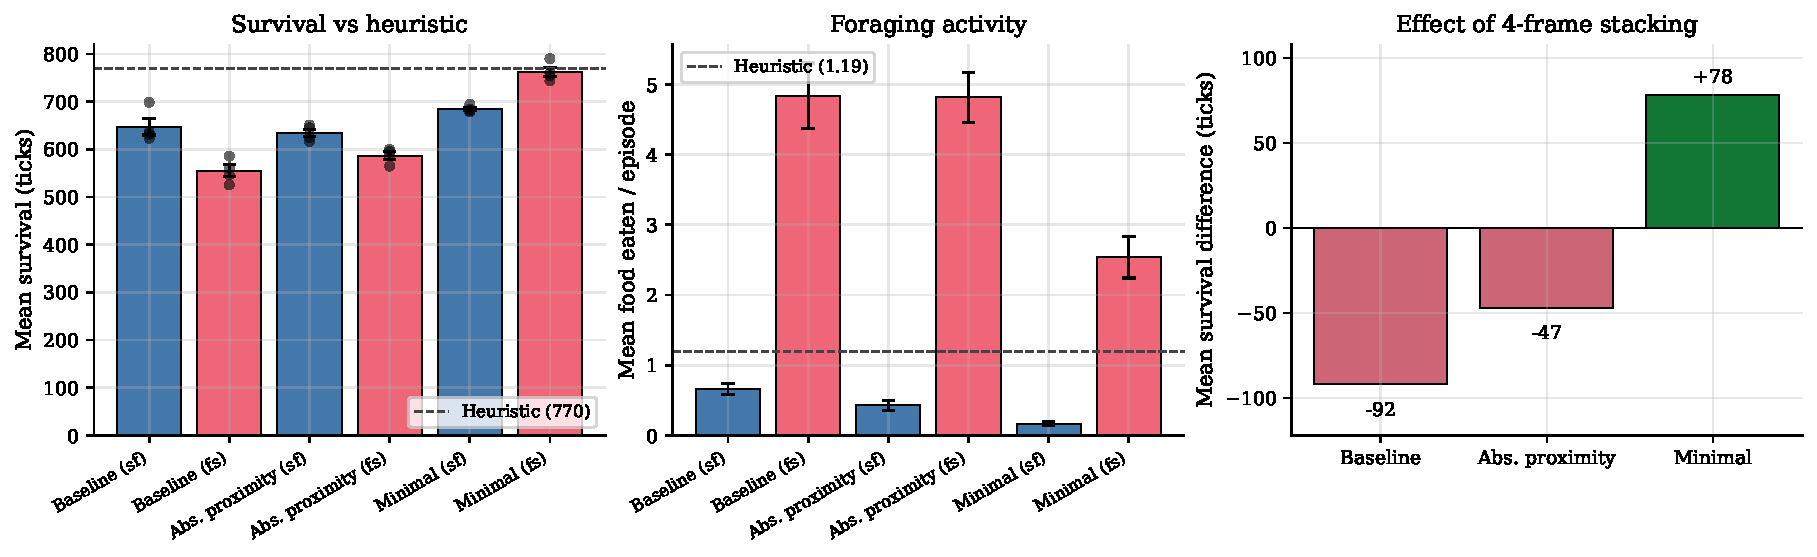
\includegraphics[width=\linewidth]{figures/ablation_grid}
\caption{Reward $\times$ observation ablation. Each bar in the first two panels is the mean over four seeds. Black dots show individual seeds. Error bars are the standard error of the mean. Dashed lines mark the heuristic baseline ($769$ ticks survival, $1.19$ food per episode). The third panel shows the mean change in survival between the single-frame and 4-frame configurations of each reward.}
\label{fig:ablation_grid}
\end{figure}

\begin{table}[!ht]
\centering
\caption{Reward $\times$ observation ablation. Each cell aggregates four seeds ($42$, $43$, $44$, $45$). ``Paired diff vs heur'' is the cell mean (over training seeds) minus the heuristic, averaged across the $100$ matched evaluation worlds, with the $95\%$ confidence interval on that difference in brackets. \textsc{weak\_proximity} is a single-seed reference and is reported separately. The \textsc{minimal} cells (sf and fs) are evaluated at the $50{,}000$-tick cap and paired with the heuristic at the same cap. All other cells are evaluated at the $1{,}000$-tick cap. See Section~\ref{sec:setup} for the rationale.}

\label{tab:cell_results}
\footnotesize
\setlength{\tabcolsep}{4pt}
\begin{tabular}{lrrrl}
\toprule
Cell & Survival (mean) & Food & Death rate & Paired diff vs heur ($95\%$ CI) \\
\midrule
Heuristic                          & $769 \pm 19$       & $1.19$ & $94\%$  & --- \\
\midrule
\multicolumn{5}{l}{\textit{Single-frame ($k=1$)}} \\
\textsc{baseline}                  & $647$              & $0.66$ & $98\%$  & $-122\;[-149,\,-94]$ \\
\textsc{absolute\_proximity}       & $634$              & $0.43$ & $100\%$ & $-135\;[-166,\,-103]$ \\
\textsc{minimal}                   & $684$              & $0.17$ & $100\%$ & $-88\;[-111,\,-64]$ \\
\midrule
\multicolumn{5}{l}{\textit{4-frame stacked ($k=4$)}} \\
\textsc{baseline\_fs}              & $555$              & $4.83$ & $97\%$  & $-214\;[-242,\,-187]$ \\
\textsc{absolute\_proximity\_fs}   & $587$              & $4.82$ & $96\%$  & $-182\;[-209,\,-155]$ \\
\textsc{minimal\_fs}               & $\mathbf{762}$     & $2.54$ & $100\%$ & $\mathbf{-10\;[-36,\,+16]}$ \\
\midrule
\textsc{weak\_proximity} (1 seed)  & $647$              & $0.66$ & $99\%$  & \textit{n/a (single seed)} \\
\bottomrule
\end{tabular}
\end{table}

Prediction P1 held. Mean survival across the six cells ranges from $555$ (\textsc{baseline\_fs}) to $762$ (\textsc{minimal\_fs}), and \textsc{minimal\_fs} is the only cell that comes close to the heuristic. The second-best cell is \textsc{minimal} (single-frame) at $684$ ticks, trailing by $78$ ticks. The within-cell standard error of \textsc{minimal\_fs} is small enough that no other cell is consistent with matching its mean.

P2 is not affirmed. Frame stacking lifts \textsc{minimal} from $684$ to $762$ ticks, but the paired gap to the heuristic is $-10.0$ ticks ($95\%$ CI $[-36, +16]$, $p = 0.45$). The confidence interval includes zero, so \textsc{minimal\_fs} could be tied with the heuristic, but we cannot show that it exceeds the heuristic. The original aim of the project was to raise DQN survival to or beyond the heuristic's level, and the data are consistent with that aim being met within statistical noise rather than affirming a clear excess.

Before turning to P3, the spread of the single-frame row is itself worth noting. The three single-frame cells span only about $40$ ticks of survival ($634$ for \textsc{absolute\_proximity}, $647$ for \textsc{baseline}, $684$ for \textsc{minimal}), and all three fall below the heuristic at $p < 0.001$. Reward configuration matters marginally in this row, but not enough to bring DQN within reach of the heuristic without temporal context.

P3 did not hold, and the direction flipped. With $\Delta = \text{mean}(\text{fs}) - \text{mean}(\text{sf})$, we observe $\Delta = +78$ for \textsc{minimal}, $\Delta = -47$ for \textsc{absolute\_proximity}, and $\Delta = -92$ for \textsc{baseline} (Figure~\ref{fig:ablation_grid}, third panel). Frame stacking helps the cleanest reward and hurts the two leakier ones, both by margins much larger than within-cell variance. In principle, additional observation channels should weakly improve the agent, since extra information can be ignored if it is not useful. The data are inconsistent with this expectation, and this flip is the largest departure from our priors and motivates the rest of the discussion.

The obvious first explanation for the leaky-cell degradation is capacity. The observation grows $3.99\times$ while the network is held fixed, so the frame-stacked agent could simply be under-provisioned. But that explanation is reward-independent, and would thus predict uniform degradation across the three rewards, whereas the observed effect flips sign with reward shape and \textsc{minimal\_fs} is the strongest cell in the study. The effect of frame stacking is mediated by the reward, not the architecture.

While the flip cannot be explained by capacity, the episode return clarifies the mechanism. Within each reward configuration,  the reward function is identical across $k$, so episode return is directly comparable across observation types. Frame stacking raises mean return on both leaky rewards (by about $+38$ on \textsc{baseline} and $+17$ on \textsc{absolute\_proximity}) while lowering survival. On \textsc{minimal} the return is essentially unchanged across $k$ (it sits near $-10$ regardless of $k$, since the minimal reward is closeness-change proximity rewards plus a terminal death penalty, neither of which scales with episode length) and survival rises. Figure~\ref{fig:return_vs_survival} plots the frame-stacking delta in return against the delta in survival for each reward. The two leakier rewards land in the lower-right quadrant where return rises and survival falls, the geometric signature of the agent collecting more reward while staying alive less long. \textsc{minimal} sits on the y-axis with a positive survival shift and essentially no return shift. Under the leaky rewards, the frame-stacked agent is more effective at collecting reward than the single-frame agent, but at the cost of survival. The reward function is misaligned with survival, and the agent is faithfully optimizing it. This is the pattern of capability-driven reward hacking \citep{Pan2022}.

\begin{figure}[t]
\centering
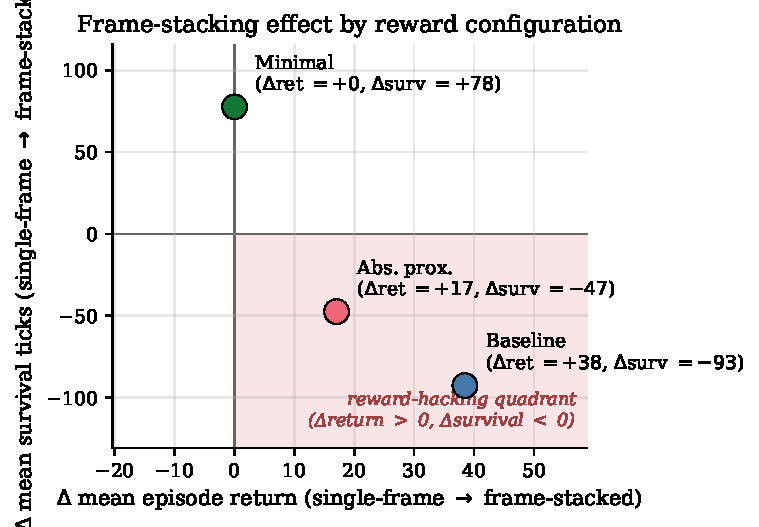
\includegraphics[width=0.78\linewidth]{figures/return_vs_survival}
\caption{Frame-stacking effect on mean episode return (x-axis) and mean survival ticks (y-axis), one point per reward configuration. Each point is the (sf $\to$ fs) shift in the per-cell means, averaged across the four training seeds and $100$ evaluation worlds. The shaded lower-right region marks the reward-hacking quadrant where return rises and survival falls.}
\label{fig:return_vs_survival}
\end{figure}

The pattern we observe is one instance of the reward-capability interaction documented across four richer environments by \citet{Pan2022}. The frame-stack increase from $k=1$ to $k=4$ functions as a capability axis comparable to those they study (model capacity, action-space resolution, observation noise, and training time), and our two leaky reward configurations exhibit the same direction they document across all of theirs. More capability brings higher proxy reward and lower true reward, and frame stacking exposes the exploitable surplus in the leakier reward designs.

Pan et al.\ additionally identify \emph{phase transitions}, ``capability thresholds at which the agent's behavior qualitatively shifts, leading to a sharp decrease in the true reward.'' Our experimental design varies frame stacking only between $k=1$ and $k=4$ and is therefore insufficient to resolve whether the survival drop is smooth in $k$ or has a phase-transition structure at some intermediate value. The broader implication for reward-design practice is that a reward function that looks adequate at one level of agent capability may produce a qualitatively different policy at another, particularly in applied settings where the true reward is observed only sporadically and the proxy is what is trained against.

\subsection{Behavior at evaluation}
\label{sec:behavior_eval}

To characterize what each cell is doing beyond aggregate survival, we separate how episodes end from what the agent does with its time. Every episode either reaches the time cap or ends in death, and every death is attributed to its terminal damage, which is either enemy contact or starvation. Deaths to enemy contact are split further by the agent's behavior over the \emph{final encounter}, the unbroken run of ticks with an enemy in view that ends at death. Over that window we sum the per-tick change in distance to the nearest visible enemy caused by the agent's own move, holding enemy positions fixed within each tick so that enemy pursuit is not misattributed to the agent. A negative sum means the agent's own moves brought it closer to the enemy, and the episode counts as enemy suicide, the suicide mode of Section~\ref{sec:failure_modes}. A zero or positive sum means the agent stood still or retreated, and the episode counts as a failure to escape. This yields four mutually exclusive outcome categories (time cap, enemy suicide, failure to escape, starvation), shown in Figure~\ref{fig:failure_modes}, with exact percentages in Appendix~\ref{app:failure_modes}.

\begin{figure}[t]
\centering
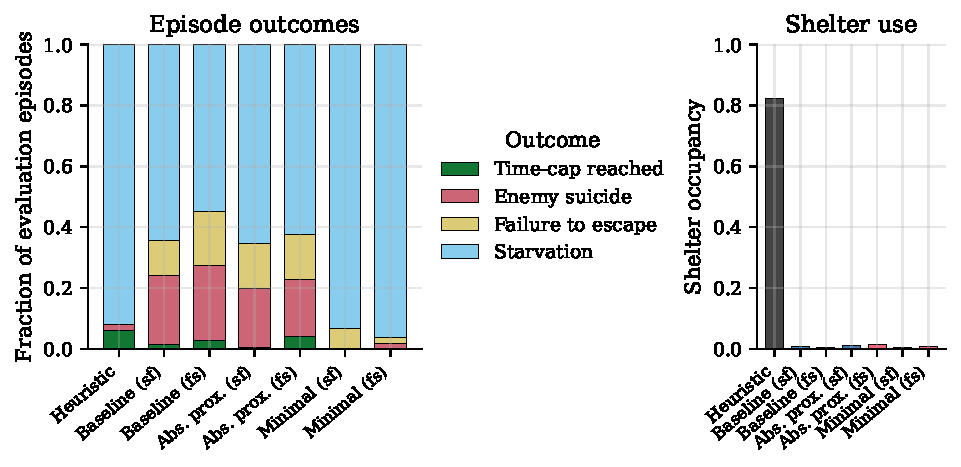
\includegraphics[width=\linewidth]{figures/failure_modes}
\caption{(Left) episode outcomes of the $100$-episode benchmark, averaged across the four seeds for each cell. Every episode reaches the time cap or ends in death from enemy contact or starvation. Enemy deaths split into enemy suicide (the agent's own moves brought it closer to the enemy over the final encounter) and failure to escape (it retreated or stood still). (Right) mean shelter occupancy (fraction of survived ticks spent inside a shelter). The heuristic spends $\approx 82\%$ of its life in shelters. Every DQN cell spends $<2\%$ regardless of reward configuration.}
\label{fig:failure_modes}
\end{figure}

The second view is the movement composition of Table~\ref{tab:movement}, the mean fraction of episode ticks the agent spends stationary, oscillating, or moving otherwise. An oscillation tick is one where the agent repeatedly moved and undid the move ($p_t = p_{t-2}$ with $p_t \neq p_{t-1}$).

\begin{table}[!ht]
\centering
\caption{Movement composition. Mean percentage of episode ticks spent stationary, oscillating (sustained two-cell cycles, at least $A,B,A,B$), or in other movement, averaged over episodes and seeds.}
\label{tab:movement}
\small
\begin{tabular}{lrrr}
\toprule
Cell & Stationary & Oscillating & Other movement \\
\midrule
Heuristic                          & $98.1\%$ & $0.2\%$ & $1.8\%$ \\
\midrule
\textsc{baseline}                  & $90.4\%$ & $6.2\%$ & $3.5\%$ \\
\textsc{absolute\_proximity}       & $91.2\%$ & $5.9\%$ & $2.9\%$ \\
\textsc{minimal}                   & $96.0\%$ & $1.8\%$ & $2.2\%$ \\
\midrule
\textsc{baseline\_fs}              & $47.7\%$ & $7.7\%$ & $44.6\%$ \\
\textsc{absolute\_proximity\_fs}   & $51.1\%$ & $9.0\%$ & $39.9\%$ \\
\textsc{minimal\_fs}               & $78.0\%$ & $2.3\%$ & $19.8\%$ \\
\bottomrule
\end{tabular}
\end{table}

Figure~\ref{fig:trajectories} shows one representative episode per cell, plotted as the agent's position trace through the $64 \times 64$ grid. The top-row (single-frame) panels collapse to a small cluster of cells. The bottom-row (frame-stacked) panels both cover much more of the grid and show the resulting increase in food eaten.

\begin{figure}[t]
\centering
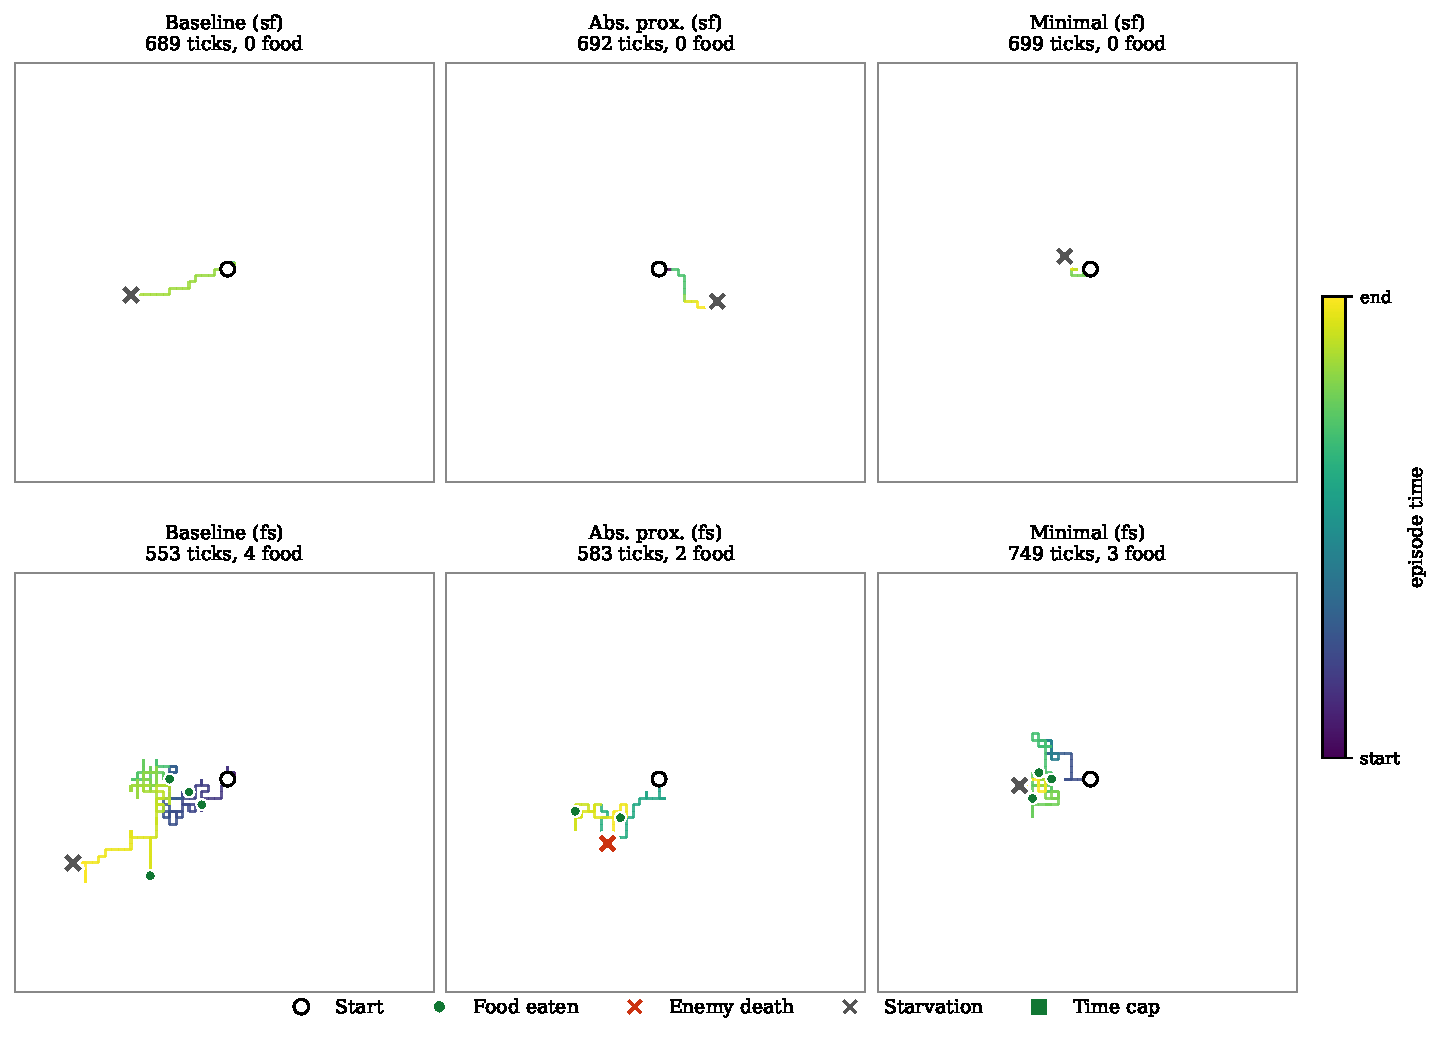
\includegraphics[width=\linewidth]{figures/trajectories}
\caption{Representative position traces, one episode per cell of the main ablation. For each cell, the episode shown is the one whose survival is closest to the cell's median across all $400$ evaluation episodes ($4$ training seeds $\times$ $100$ evaluation worlds). The path is colored by tick (light early, dark late). The start position is the open circle. Food-eaten events along the path are green dots. The end marker indicates cause of death (red ``X'' for enemy contact, gray ``X'' for starvation, green square for reaching the time cap). Food and shelter locations are not drawn, since food respawns stochastically and shelters are unoccupied in every DQN episode.}
\label{fig:trajectories}
\end{figure}

Two regularities stand out in the displayed outcomes. First, starvation is the dominant death cause everywhere, from $55$--$66\%$ of episodes in the leaky cells to $92$--$96\%$ for the heuristic and the \textsc{minimal} cells. Second, enemy suicide shows exactly what the analysis of Section~\ref{sec:failure_modes} predicted: the two leaky rewards retain the hunger-proportional and starvation penalties that make a quick death cheaper than slow starvation, and their cells show $19$--$25\%$ enemy suicide, with every one of the sixteen leaky-cell seeds between $12\%$ and $39\%$. \textsc{minimal} zeroes those penalties, equalizing the reward cost of fast and slow death, and its suicide rate is $0\%$ single-frame and $1.8\%$ frame-stacked.

The movement composition captures what the outcomes barely register, namely the effect of frame stacking. Within each reward, the outcome mix changes only modestly from $k=1$ to $k=4$, but the movement mix transforms. The single-frame cells spend $90$--$96\%$ of their ticks stationary, even more immobile than the heuristic ($98\%$), which at least stands still inside shelters. With frame stacking, stationary ticks fall to $48$--$51\%$ in the leaky cells and $78\%$ in \textsc{minimal}, and most of the freed time goes to genuine movement rather than oscillation. Oscillation is a minor pattern everywhere, at most $9\%$ of ticks (\textsc{absolute\_proximity\_fs}), so exposed stasis in this environment is overwhelmingly standing still rather than cycling in place. In short, the two axes act on different aspects of behavior. Outcomes follow the reward: the leaky cells differ from \textsc{minimal} in their suicide and starvation shares at both observation depths, while going from $k=1$ to $k=4$ barely changes the outcome mix within a reward. Movement follows the observation: stationary time falls under frame stacking for every reward. The two axes still interact in the size of that fall: about $40$ percentage points under the leaky rewards against $18$ under \textsc{minimal}, which leaves \textsc{minimal\_fs} far more stationary ($78\%$) than the leaky frame-stacked cells ($48$--$51\%$), consistent with its higher survival, since exposure scales with time spent moving in the open.

The added movement is productive foraging, not wandering. Food per episode rises from $0.17$ to $2.54$ for \textsc{minimal}, from $0.43$ to $4.82$ for \textsc{absolute\_proximity}, and from $0.66$ to $4.83$ for \textsc{baseline}. With frame stacking, the agent learns to follow the food-proximity reward more aggressively, but in the leaky reward configurations the resulting policy spends more ticks exposed to enemies and dies sooner. Foraging behavior is acquired and safety behavior is not. Only \textsc{minimal\_fs} reaches a foraging rate consistent with sustained survival ($2.54$ food per episode at survival within $10$ ticks of the heuristic, against the heuristic's $1.19$ food at $769$ ticks).

Foraging is one half of the heuristic's strategy. Shelter use is the other half, and it is essentially absent across all six DQN cells (median $0.9\%$ of survived ticks, max $1.4\%$ for \textsc{absolute\_proximity\_fs}, driven largely by one outlier seed averaging $3.0\%$ over its $100$ episodes while the other three sat at $0.5$--$1.6\%$). No cell has learned to use the shelters as the heuristic does at $82\%$.

For the \textsc{minimal} configuration this is informative, because the reward was specifically designed to teach the heuristic's shelter mode via a shelter-proximity reward gated on hunger $\geq u_\text{gate}$ (Section~\ref{sec:reward_configs}). One plausible hypothesis is that the gate never opens, in which case the agent's hunger stays below $u_\text{gate} = 0.5$ for most of the episode and the shelter-proximity reward never fires. To test this, we logged the agent's hunger ratio at every tick and ran the four trained \textsc{minimal\_fs} checkpoints on the $100$-world evaluation suite. Across these $400$ episodes the agent's hunger was at or above $u_\text{gate}$ for a mean of $32.0\%$ of episode ticks (longest continuous open-gate streak averaged $237$ ticks per episode, median $249$, max $324$), and all $400$ episodes started above the gate since the agent begins every episode at full hunger. The gate is therefore open often enough and for long enough that the shelter-proximity reward has substantial opportunity to fire, and this hypothesis is rejected.

An alternative explanation is that the $\Delta\phi$ formulation of the shelter-proximity reward pays only for approaching a shelter, not for occupying one. Once the agent is inside a shelter the closeness no longer changes, so $\Delta\phi^{(s)} = 0$ on every subsequent tick, and the shelter-safety reward $w_\text{shelter}$, which pays for occupancy directly, is zero in the present \textsc{minimal} configuration (Table~\ref{tab:minimal_config}). On its own this cannot explain the gap, because the four misspecified cells keep $w_\text{shelter}$ at its default $+0.1$ and show the same near-zero occupancy. What no cell provides is both halves at once. The misspecified rewards pay for being sheltered but give no directional signal for finding a shelter, so the agent could only discover the payment through undirected exploration, and the payment itself fires only when an enemy is within distance $3$ of the sheltered agent (Table~\ref{tab:default_rewards}), an event a passing shelter visit rarely triggers. \textsc{minimal} on the other hand gives the directional signal, but pays nothing for staying.

Finally, shelter use may not even be strictly necessary for survival in this environment, since the enemy density and pursuit rules of Section~\ref{sec:world_design} may simply not impose enough damage pressure to make shelter-camping a required strategy. The fact that \textsc{minimal\_fs} reaches $762$ ticks, similar to the heuristic, without any shelter use supports this possibility.

Beyond the shelter question, the \textsc{baseline} versus \textsc{absolute\_proximity} contrast isolates the effect of the closeness-change reward shape. At single-frame, switching the proximity term from $\Delta\phi$ to $\phi$ degrades survival by $13$ ticks ($647 \to 634$) and lowers food intake from $0.66$ to $0.43$ per episode. The lower food intake is consistent with the agent earning proximity reward for being near food without crossing onto the food tile to eat it. At frame-stacked, the same switch improves survival by $32$ ticks ($555 \to 587$) with essentially unchanged food intake ($4.83 \to 4.82$). The 4-frame stack appears to give the agent enough temporal information to navigate onto food rather than hover next to it, so the absolute form is no worse than the closeness-change form at this observation level. The closeness-change form, used in \textsc{minimal}, remains the only reward shape under which frame stacking improves survival relative to its own single-frame counterpart.

\subsection{Learning dynamics}
\label{sec:learning_dynamics}

Figure~\ref{fig:learning_curves} plots the in-training $100$-episode evaluation survival as a function of training step for each of the six ablation cells. The trajectories support three observations relevant to the experimental design. First, each cell's curve flattens by step $1.0$--$1.4$M, and the second half of training contributes drift rather than a discernible upward trend in any cell. Because of this, we terminate training at $T = 2{,}000{,}000$ steps. We cannot rule out ``grokking'', a sudden jump in survival after long stagnation~\citep{Power2022} or a slow but steady improvement past this budget. Second, the trajectories are tightly clustered across seeds within a cell, which corroborates the per-seed survival homogeneity reported in Table~\ref{tab:per_seed} and indicates that the variance across cells is attributable to (reward, observation) variation rather than random initialization. Third, the displayed values use a $10$-eval trailing mean (partial window for the first 9 evals) over $100$ episodes per eval, so they track the $100$-episode benchmark numbers reported in Table~\ref{tab:cell_results} closely.

\begin{figure}[t]
\centering
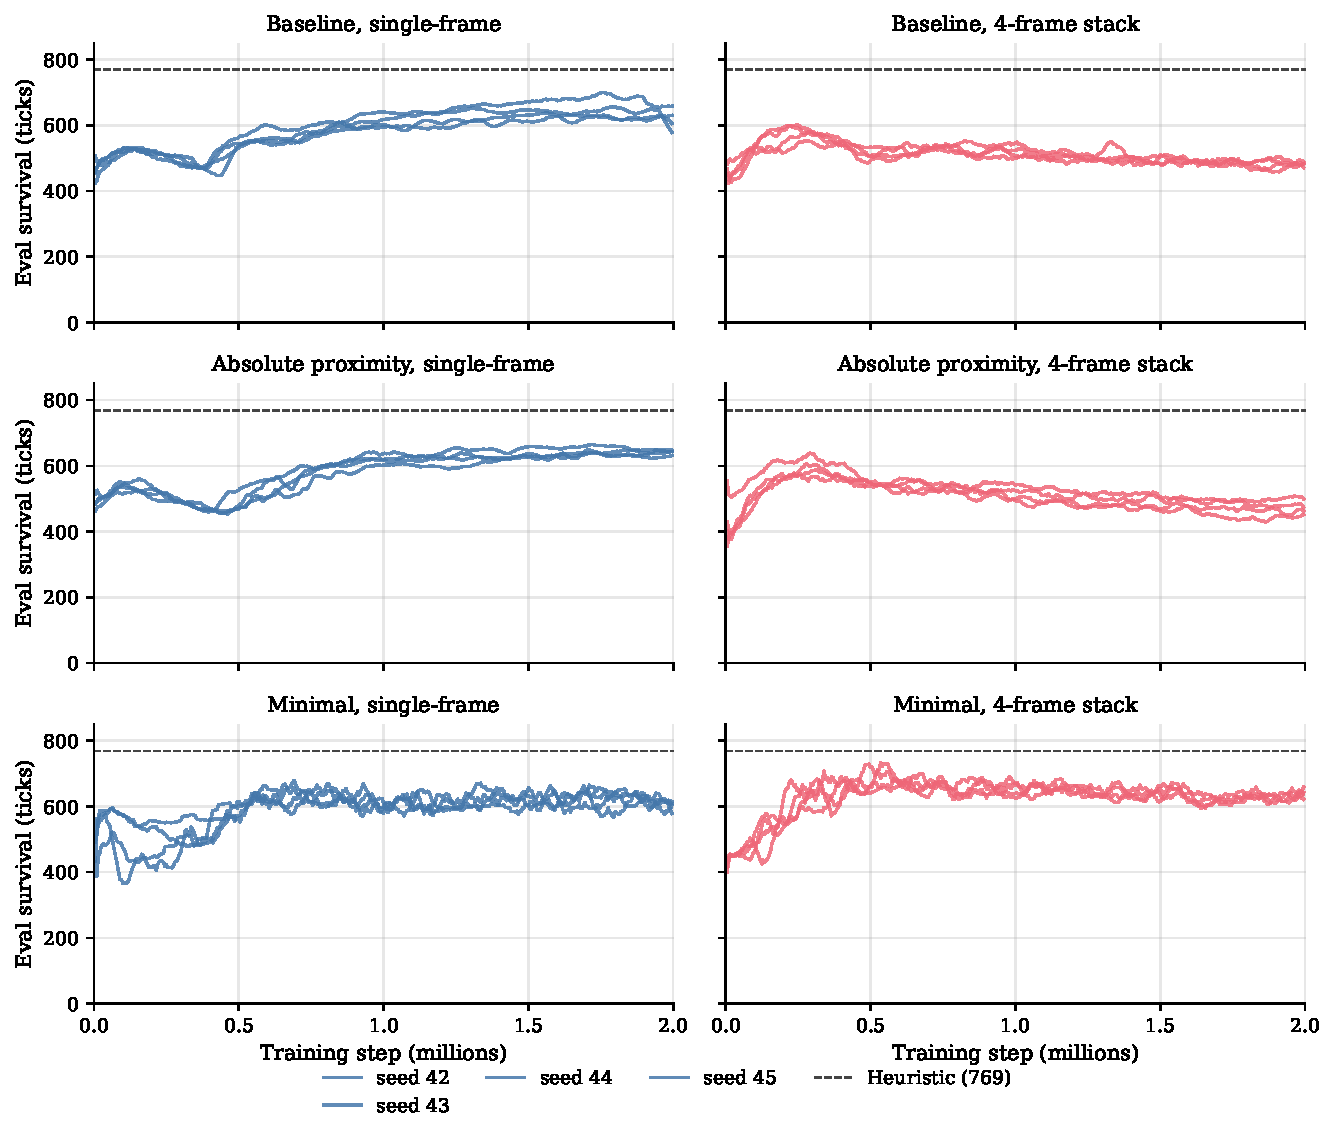
\includegraphics[width=\linewidth]{figures/learning_curves}
\caption{In-training evaluation survival vs training step for the six ablation cells. Each line is one seed, smoothed with a $10$-eval rolling mean ($50{,}000$-step window). The dashed gray line at $769$ ticks marks the heuristic baseline.}
\label{fig:learning_curves}
\end{figure}

\subsection{Limitations}
\label{sec:limitations}

The most important limitation is external validity. All findings come from a single, custom-built environment and a single task, so the numbers are not directly comparable to results reported for Crafter, MiniGrid, or other gridworld libraries, and the reward-dependent direction of the frame-stacking effect can only be generalized through replication on other environments.

The second limitation concerns the design of the reward axis itself. \textsc{minimal} differs from \textsc{baseline} in several ways at once: it removes the hunger penalties, drops the event rewards for eating and taking damage while keeping only the death penalty, activates proximity terms that \textsc{baseline} leaves disabled, gates two of them on hunger, and assigns different weights. ``Clean versus leaky'' is therefore one description of a many-dimensional change, not a single isolated factor. The return signature of Section~\ref{sec:results} supports the leak-exploitation mechanism, since under frame stacking the leaky cells collect more reward while surviving shorter, but the design cannot rule out that some other ingredient of the bundle is the actual causal variable. An ablation that removed one leak at a time, for example zeroing the hunger-proportional and starvation penalties, the pair that makes a quick death cheaper than slow starvation, while leaving the rest of \textsc{baseline} intact, would isolate the mechanism more sharply.

Three further constraints qualify the strength of the claims. First, the network architecture is held fixed across observation depths, so we do not run an architecture sweep. The reward evidence in Section~\ref{sec:results} rules out an undersized $k=4$ network as the driver of the leaky-cell degradation (the effect flips sign with reward shape, and the leaky cells gain reward rather than lose it, neither of which an under-provisioned agent would do), but training the $k=4$ cells with a network scaled to their larger input would confirm this more directly. Second, the computational budget limited each cell to two million training steps. The learning curves flatten well before this point, but longer training could test whether certain configurations improve further. Third, each cell uses four training seeds, below the five to ten typically recommended in RL methodology work \citep{Henderson2018, Colas2018}. The within-cell standard errors in Table~\ref{tab:cell_results} are computed from this small sample and therefore carry substantial estimation noise themselves. A larger seed budget would estimate each cell mean more precisely and show more directly whether the survival differences between the single-frame and frame-stacked variants hold up when training is repeated with new random seeds. Finally, \textsc{weak\_proximity} was trained on a single seed, so we draw no conclusions from it beyond the qualitative note in Section~\ref{sec:weak_prox}.

% =============================================================================
\section{Conclusion}
\label{sec:conclusion}
% =============================================================================

We ran a $3 \times 2 \times 4$ ablation that crossed three reward configurations (\textsc{baseline}, \textsc{absolute\_proximity}, \textsc{minimal}) with two observation types (single-frame and 4-frame stacked), four random seeds per cell. We added a single-seed illustrative run of \textsc{weak\_proximity} to demonstrate the suicide failure mode under a too-small proximity weight.

We established three predictions: that \textsc{minimal\_fs} would be the best-performing cell (P1), that it would exceed the heuristic (P2), and that frame stacking would improve every reward configuration over its single-frame counterpart (P3). P1 held. \textsc{minimal\_fs} reaches mean survival $762$ ticks, the highest of any cell. P2 is not rejected but also not affirmed. The paired gap to the heuristic is $-10.0$ ticks ($95\%$ CI $[-36, +16]$, $p = 0.45$), so \textsc{minimal\_fs} could be tied with the heuristic but we cannot show it exceeds the heuristic. P3 did not hold: while frame stacking improves \textsc{minimal} ($+78$ ticks), it degrades \textsc{absolute\_proximity} ($-47$) and \textsc{baseline} ($-92$). 

Beyond refuting P3, the data reveal a directional structure to frame stacking's effect. It improves the cleanest reward configuration and degrades both leakier ones, by margins much larger than within-cell variance. Although we did not set out to test this, it emerged from the ablation, and is the most directly informative result of the work. It showed that adding observation history is not an unconditional improvement on this task, and that under the two leakier reward designs studied here, it even actively hurt the resulting agent. We discussed plausible mechanisms in Section~\ref{sec:discussion}.

This work studies the reward $\times$ observation interaction in DQN on one specific environment. The main contribution is the $3 \times 2 \times 4$ ablation just described, which tests three pre-specified predictions and reveals that the sign of the frame-stacking effect depends on reward shape. A second finding confirms that for the two rewards that make a quick death cheaper than slow starvation, $19$--$25\%$ of evaluation episodes end with the agent closing distance on the enemy that kills it, while \textsc{minimal}, which equalizes the reward cost of fast and slow death, shows at most $2\%$.

As a secondary outcome, the leaky-reward results corroborate the reward-capability interaction of \citet{Pan2022} in a new setting: the same direction they document across model size, action-space resolution, observation noise, and training time also appears when capability is varied through observation history, in a different environment. We do not, however, resolve whether the survival drop has the phase-transition structure they report, since our design varies $k$ at only two levels.

\label{sec:future_work}
Four directions follow naturally from these results. First, replicate the ablation on a second multi-objective environment (for example a forked MiniGrid or Crafter setup) to test the generality of the reward-dependent direction. Second, train the $k=4$ cells with a network scaled up to match the larger input. The current architecture is the same for $k=1$ and $k=4$, despite the $k=4$ observation being roughly four times the size of the $k=1$ observation. Scaling up the $k=4$ DQN agent to match the input size would help confirm that reward design, not missing capacity, explains the decrease in survival. Third, train all cells for substantially longer than two million steps to test for further survival improvements. Fourth, test whether adding a shelter occupancy reward to \textsc{minimal} produces learned shelter use. \textsc{minimal} would then be the first cell to combine a directional signal for finding shelters with a payment for staying in one, the combination Section~\ref{sec:behavior_eval} identifies as untested.

% =============================================================================
% Appendix
% =============================================================================
\newpage
\appendix

\section{Hyperparameters}
\label{app:hyperparams}

Table~\ref{tab:hyperparams} lists all agent and training hyperparameters used across the ablation. Values follow established defaults from the literature rather than environment-specific tuning. The frame-stack size $k$ is the only varying parameter, all others are held constant across all twenty-four ablation runs.

\begin{table}[!ht]
\centering
\caption{Agent hyperparameters.}
\label{tab:hyperparams}
\small
\begin{tabular}{lll}
\toprule
Parameter & Value & Reference \\
\midrule
\multicolumn{3}{l}{\textit{Optimization}} \\
Learning rate              & $10^{-4}$         & \\
Weight decay               & $10^{-4}$         & after \citet{Loshchilov2019} \\
Batch size                 & 128               & \\
Gradient clip norm         & 1.0               & \\
\midrule
\multicolumn{3}{l}{\textit{Replay buffer}} \\
Buffer capacity            & 250{,}000         & \\
Min.\ buffer size (warmup) & 10{,}000          & after \citet{Mnih2015} \\
PER $\alpha$               & 0.6               & \citet{Schaul2016} \\
PER $\beta_0$              & 0.4               & \citet{Schaul2016} \\
$\beta$ annealing steps    & $500{,}000$             & \\
$n$-step returns           & 3                 & \citet{Hessel2018} \\
\midrule
\multicolumn{3}{l}{\textit{Target network}} \\
Polyak $\tau$              & 0.002             & after \citet{Lillicrap2016} \\
\midrule
\multicolumn{3}{l}{\textit{Exploration}} \\
$\varepsilon$ start / end  & 1.0 / 0.01        & after \citet{Mnih2015} \\
$\varepsilon$ decay steps  & 500{,}000         & \\
\midrule
\multicolumn{3}{l}{\textit{Network}} \\
CNN channels               & (32, 64, 64)      & \citet{Mnih2015} \\
CNN kernel sizes           & ($3{\times}3$, $3{\times}3$, $3{\times}3$) & \\
CNN strides                & (1, 1, 2)         & \\
CNN padding                & (1, 1, 0)         & \\
Normalization              & LayerNorm         & \citet{Ba2016} \\
Merge hidden dim           & 256               & \\
Dueling head hidden dim    & 128               & \\
\midrule
\multicolumn{3}{l}{\textit{Observation (ablation variable)}} \\
Frame stack $k$            & $\{1, 4\}$        & \citet{Mnih2015} \\
\midrule
\multicolumn{3}{l}{\textit{Training}} \\
Discount $\gamma$          & 0.99              & \\
Total timesteps $T$        & 2{,}000{,}000     & \\
Eval frequency             & 5{,}000 steps     & \\
Eval episodes (in-training) & 100               & \\
Final benchmark episodes   & 100 (seeds 1000--1099) & \\
\bottomrule
\end{tabular}
\end{table}

The convolutional encoder reduces the $15 \times 15$ spatial grid to $7 \times 7$ at the third layer, producing a 3136-dimensional feature vector. This is concatenated with the three scalar observations and projected through the merge layer to a 256-dimensional representation. LayerNorm is applied after the first two convolutions and after the merge layer. The Dueling head splits this representation into a value stream ($256 \to 128 \to 1$) and an advantage stream ($256 \to 128 \to 5$), and $Q$-values are computed as $Q(s, a) = V(s) + A(s, a) - \bar{A}(s)$. For the 4-frame stacked cells ($k = 4$), the only structural change is the input depth of the first convolution ($12 \to 32$ instead of $3 \to 32$).

\section{Per-seed survival}
\label{app:per_seed}

\begin{table}[!ht]
\centering
\caption{Per-seed DQN survival (mean over the $100$-episode benchmark per seed). Heuristic survival is $769 \pm 19$ ticks. Cell-level uncertainty and the comparison to the heuristic are in Table~\ref{tab:cell_results}.}
\label{tab:per_seed}
\footnotesize
\begin{tabular}{lrrrr}
\toprule
Cell                              & seed 42 & seed 43 & seed 44 & seed 45 \\
\midrule
\textsc{baseline}                 & $623$ & $698$ & $631$ & $636$ \\
\textsc{baseline\_fs}             & $561$ & $526$ & $546$ & $586$ \\
\textsc{absolute\_proximity}      & $625$ & $651$ & $645$ & $616$ \\
\textsc{absolute\_proximity\_fs}  & $564$ & $587$ & $595$ & $600$ \\
\textsc{minimal}                  & $684$ & $681$ & $678$ & $694$ \\
\textsc{minimal\_fs}              & $755$ & $760$ & $790$ & $744$ \\
\bottomrule
\end{tabular}
\end{table}

\section{Episode outcomes and shelter occupancy}
\label{app:failure_modes}

\begin{table}[!ht]
\centering
\caption{Per-cell episode outcomes and shelter occupancy, in percent. Outcomes are mutually exclusive and sum to $100\%$ within rounding. ``Sh.\ occ.'' is the mean fraction of survived ticks spent inside a shelter, expressed as a percentage. Each row averages four seeds (the heuristic row is a single $100$-episode run).}
\label{tab:outcomes}
\footnotesize
\setlength{\tabcolsep}{4pt}
\begin{tabular}{lrrrrr}
\toprule
Cell & Cap & Enemy suicide & Failure to escape & Starvation & Sh.\ occ. \\
\midrule
Heuristic                          & $6.0$ & $2.0$ & $0.0$ & $\mathbf{92.0}$ & $82.1$ \\
\midrule
\multicolumn{6}{l}{\textit{Single-frame ($k=1$)}} \\
\textsc{baseline}                  & $1.5$ & $22.5$ & $11.5$ & $\mathbf{64.5}$ & $0.9$ \\
\textsc{absolute\_proximity}       & $0.5$ & $19.5$ & $14.5$ & $\mathbf{65.5}$ & $1.0$ \\
\textsc{minimal}                   & $0.0$ & $0.0$  & $6.8$  & $\mathbf{93.2}$ & $0.6$ \\
\midrule
\multicolumn{6}{l}{\textit{4-frame stacked ($k=4$)}} \\
\textsc{baseline\_fs}              & $2.8$ & $24.8$ & $17.8$ & $\mathbf{54.8}$ & $0.6$ \\
\textsc{absolute\_proximity\_fs}   & $4.2$ & $18.5$ & $14.8$ & $\mathbf{62.5}$ & $1.4$ \\
\textsc{minimal\_fs}               & $0.0$ & $1.8$  & $2.0$  & $\mathbf{96.2}$ & $1.0$ \\
\bottomrule
\end{tabular}
\end{table}

% =============================================================================
% References
% =============================================================================
\newpage
\bibliographystyle{plainnat}
\bibliography{refs}

\end{document}
